\glsresetall{} 

\chapter{Software Architecture}\label{chap:architecture}

\lettrine[lines=2, findent=0pt, nindent=5pt]{T}{}he \gls{pops} is made up of
several distinct components separated into services.  The reason it has been
separated in this way, is to allow for separation of concerns. That being, each
functional unit of the tool is separated with limited overlap. Developing in
this way allows for a great deal of freedom when developing the different
services of the tool. Each service will be completely unaffected by the
implementation of another service. In addition, some of the functionality of
\gls{pops} has functionality that is useful outside of the tool itself. Through
this architecture, the services may be used elsewhere, without any need for
further development for the services.  

Each service has its own Docker container. Containers are similar to virtual
machines in that they simulate an operating system but, unlike virtual
machines, they do not simulate the underlying hardware. This makes containers
much more lightweight, while also retaining the benefits of having a
standardized environment where dependencies are packaged with their source
code. Containers make deploying and maintaining \gls{pops} much easier since
installation does not require managing dependencies and tweaking environment
variables. In this way, a \gls{pops} user does not need to be as familiar with
the software as a developer to run it.  Each service is its own Python web
server. In this way, they may be interacted with via a RESTful API. That being,
HTTP requests can be made to retrieve information or perform calculations. Each
service also provides its own automatically generated documentation that can be
accessed through a web browser. This documentation outlines possible API calls
as well as their input and output data formats.  This allows a user to quickly
see the capabilities of a service without accessing the source code. Currently,
\gls{pops} has 4 main services; they are the: Mission Model, Propagator,
Database, and Access Time Utilities.

%% ======================================================================== %%
%%			    General Architecture
%% ======================================================================== %%

\section{General Service Architecture}

Every service contains the same basic components so it is worth discussing
services generally and then going into specifics in subsequent sections. These
components are: the Dockerfile, a main Python script, a models file, and
service specific scripts.

To review, a docker container is a virtual environment, which is a simulated
operating system. A container can be hosted on any operating system that
supports docker. Images are the templates that can be used to create
containers. They can either be built on the user's machine or they may be built
elsewhere and then copied onto the user's machine. Dockerfiles are the
configuration files that are used to assemble an image. They specify: the
operating system that should be used, what files should be included in the
container, and what commands should be run upon container creation. By
specifying an operating system, we can tailor a service to any environment that
best suits the service's needs.  They can use windows, the latest version of
Ubuntu, or a lightweight tailored Linux distribution that only contains the
tools a service needs. In this way, one service can be running Ubuntu 20.04
and another service can be running Windows 10. In this way, \gls{pops} is not
limited by the operating system it is developed in.  Files may be added to a
container simply by pointing to their location in the host's file system upon
image creation.  Finally, when a container is first created from an image, a
container will need to install all of the necessary dependencies. In general,
this will either be Ubuntu packages, a version of Python, and Python libraries.
In this way, dependencies can easily be tracked. 

Theoretically, all of the code for a service could live in the main Python file
but, if this were the case, it would quickly balloon and become unwieldy to
work with so functionality is split into multiple scripts. The main script's
purpose is to handle all of the webserver aspects of the service. It is a
collection of functions that handle: creating the web-server, setting server
parameters, setting up environment variables, and \gls{api} calls.  Setting up
the webserver is fairly straightforward since open source libraries are used to
handle all of the low-level functionality and implementation. What is most
important is specifying potential \gls{http} requests. These requests are how a
service may be interacted with by a user, their browser, or by other services.
The parts of an HTTP request that must be specified are the: 

\begin{itemize}
    \item Request type (GET, POST, DELETE, PUT, etc.), 
    \item Path to the request, 
    \item Response type (JSON, Plain Text, HTML, None, etc.), 
    \item Input variables (if applicable), and the 
    \item Function that is called when a request is received.
\end{itemize}

\gls{http} supports 5 main types of request: GET, POST, DELETE, PUT, and PATCH.
\gls{http} does not for the most part impose restrictions on what a request can
do. These types are useful for organizational purposes but do not need to be
strictly conformed with. For large applications they are useful, but \gls{pops}
generally only makes use of the first 3.  For GET requests, there is no payload
so the only information that is transferred is the link itself or any query
parameters.  These requests are used to read information from the webserver
such as a webpage or some specific data. DELETE requests are equivalent to GET
requests but they are used when information must be deleted from \gls{pops}.
Given how important potential data loss is, deletions are treated separately.
POST requests contain information in the body of the request.  The format of
the input data must be defined or else the web server will fail the request as
being unprocessable.  These input definitions are stored in the models file.
Python is a dynamically typed language so variables do not need to be assigned
a type upon creation. To ensure input data conforms with what is expected by
the \gls{api}, the Python library, \texttt{Pydantic}, is used to enforce data
types at runtime.  These Pydantic input definitions are contained in the models
file.  The remainder of the files in a service are specific to the service
itself.

Having multiple Docker containers becomes cumbersome when a user or a developer
wishes to build new images or run new containers from their images. To manage
all of the different services, another tool is used called "Docker Compose".
From a single configuration file, multiple services may be started, stopped, or
built from their source code. Services may also have their image name,
container name, and port number set through the configuration file. This vastly
simplifies configuration for \gls{pops} as a whole. Another benefit of using
Docker Compose is that it also creates a bride network for the containers
Docker Compose creates. Containers are intended to be standalone units but a
bridge network allows containers to communicate with each other directly
without them needing to keep track of the IP they are hosted on.

%% ======================================================================== %%
%%			    Propagator
%% ======================================================================== %%

\section{Propagator Service}

The Propagator service handles ephemeris generation for \gls{pops}.
Ephemerides are a crucial component for every subsequent step along the
planning process so it is essential that they are well formed. Consolidating
ephemeris generation for the entire tool ensures that only one area of the code
needs to be developed and validated.

As discussed in Chapter~\ref{chap:ops}, the main method of orbital propagation
for \gls{pops} is with the \gls{sgp} model series of algorithms, specifically
SGP4/SDP4 referred to as just ‘SGP4’.  \gls{sgp4} is an analytical method of
approximating orbital state vectors at corresponding epochs in the \gls{teme}
\gls{eci} coordinate frame, given a NORAD \gls{tle}.  \gls{tle}s are readily
provided by the United States Space Force through Space-Track.  Alternatively,
\glspl{tle} may also be taken from CelesTrak which gets \glspl{tle} from
Space-Track and applies its own modifications.  The \gls{teme} coordinate frame
is not particularly useful so part of the Propagator service’s purpose is
transforming the orbit vectors into a coordinate system required by other parts
of \gls{pops}.  Currently, the two possible output reference frames are the
\gls{gcrs}, which is an \gls{eci} reference frame, and the \gls{wgs}, which is
an \gls{ecef} reference frame.  Depending on the application, it is sometimes
useful to use \gls{eci} or \gls{ecef} reference frames, so both are made
available by the service.  Given a \gls{tle}, a time range, a step size, and a
coordinate system, the Propagator service generates an Ephemeris for the
provided time range in a variety of output formats.

There are two scripts that handle all of the functionality for the Propagator
service. The first is the main script which, as discussed previously, takes
requests, organizes the input data, and formats the output data. The actual
propagation and coordinate change logic is stored in the propagation script.
Open source libraries are used to perform the SGP4 and coordinate transform
algorithms so the main focus of the script is to ensure the input data conforms
with the expected format.  

\begin{figure}[h]
    \centering
    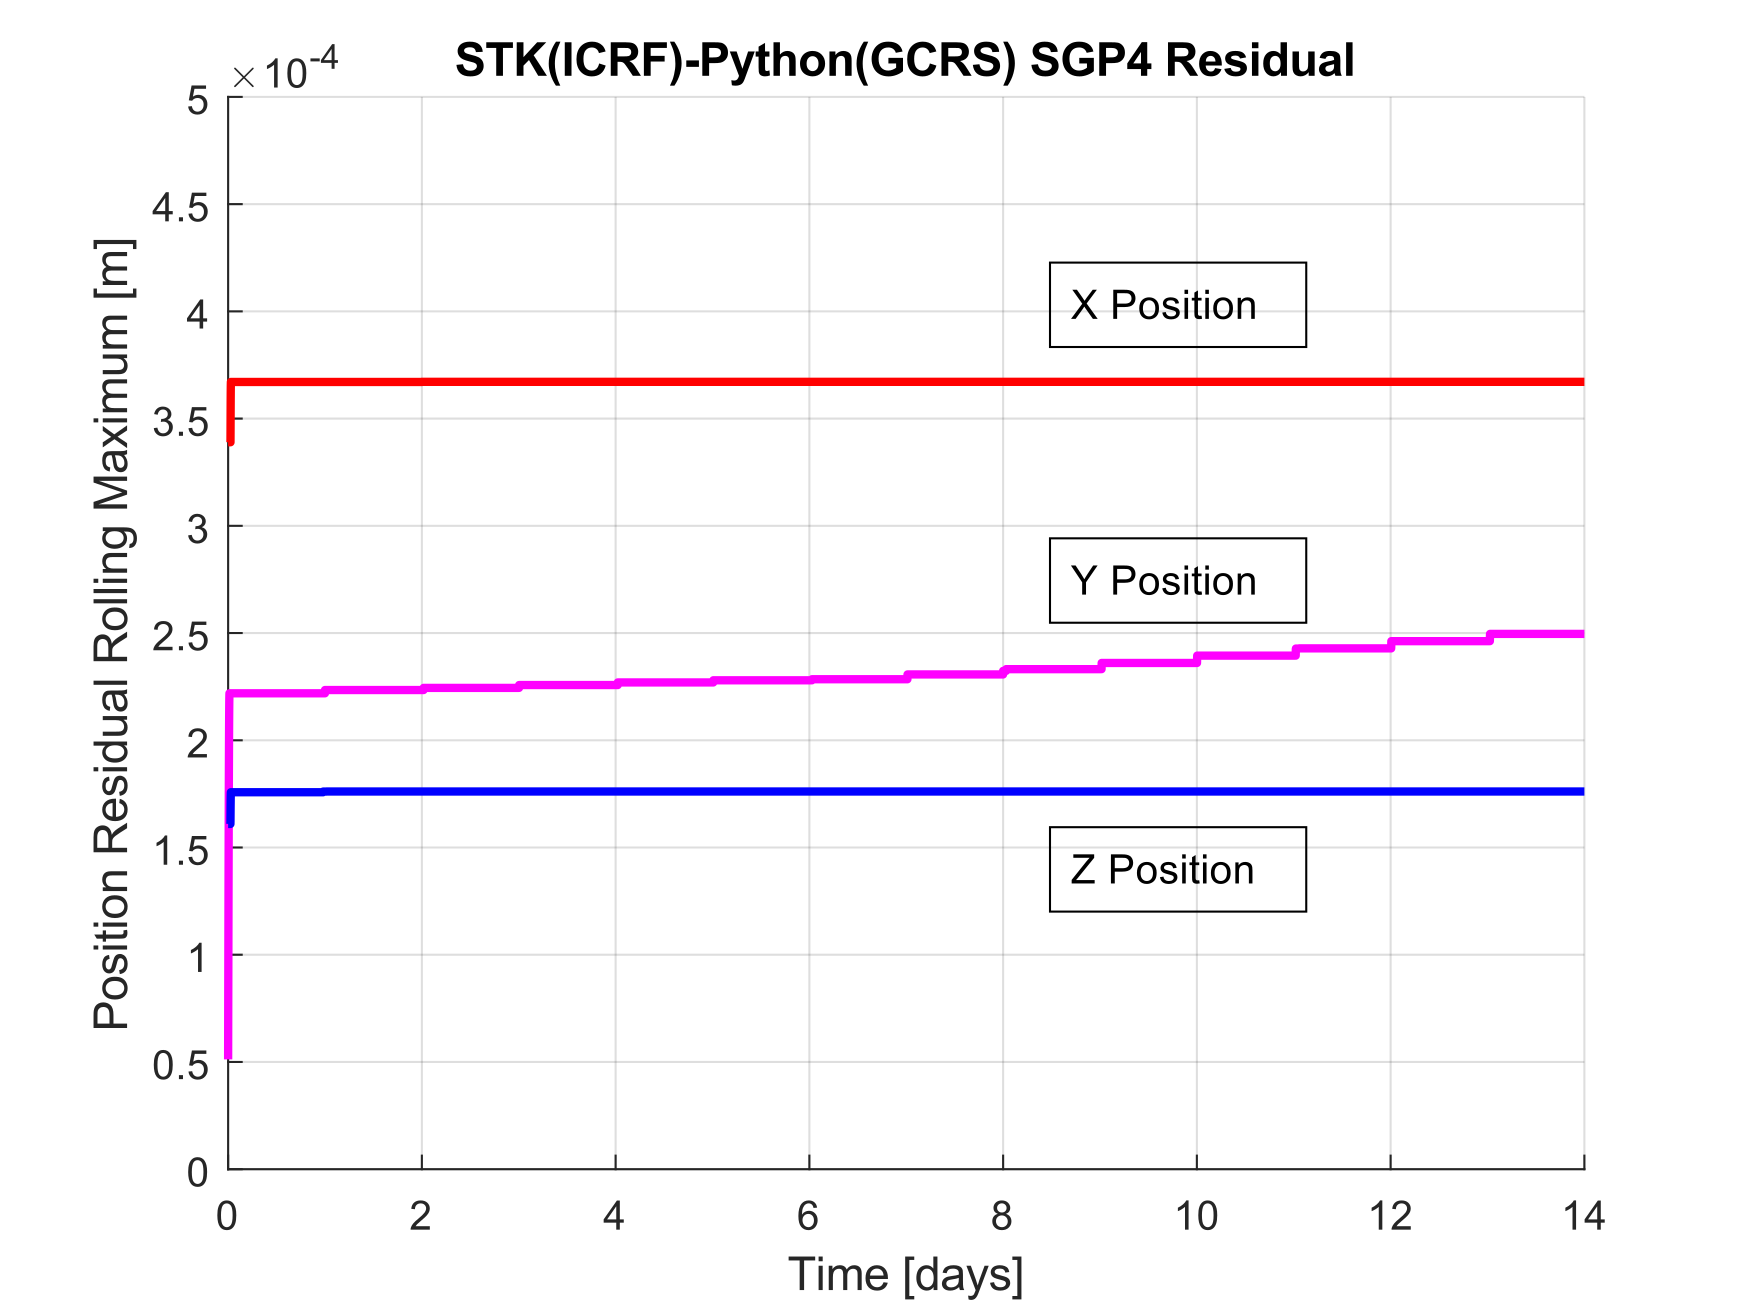
\includegraphics[width=0.7\textwidth]{STK_PY_residual-2.png} 
    \caption{Residual Difference \gls{stk} vs. Python}
    \label{fig:stk_py} 
\end{figure}

It is very easy to generate Ephemeris data. What is difficult is validating it.
The benchmark for validation is \gls{stk} since it has its own SGP4 ephemeris
generation capabilities. If operators did not use POPS, their best alternative
would be to set up scenarios manually in \gls{stk}. As such, using it as ground
truth is valid in this case. Both \gls{stk} \cite{kelso_celestrak_2022} and the
\gls{pops} implementation of SGP4 use the same source
\cite{vallado_revisiting_2006}.  As such, they should provide the same results.
One difference to note is that \gls{stk} uses the \gls{icrf} \gls{eci}
coordinate system but the propagator service uses \gls{gcrf}.  This difference
is acceptable since these reference frames are approximately identical
\cite{kaplan_iau_2006}.  The procedure for validating the Propagator service
was first to select a \gls{tle}, a time range, a time step, and a coordinate
system.  Next was to generate Ephemerides from \gls{stk} and the propagation
service.  Finally, the results were compared. One such comparison can be seen
in Figure~\ref{fig:stk_py}. Here, the peak position residual was 0.37mm for the
position along the x-axis. The main purpose of this exercise is to ensure that
the Python libraries are being used correctly and that their output data is
acceptable.  From this result, it is clear that the methods are identical and
the difference was most likely due to slight implementation differences. 

Another responsibility of the Propagator service is to determine a list of
passes for a given ephemeris. Having an entire ephemeris may be cumbersome for
some calculations so it makes sense to split a whole ephemeris into multiple
components. A `pass' is a arbitrary term so in this context it is defined as
the period between south-to-north hemisphere crossings. This definition was
chosen because it is easy to calculate when a spacecraft crosses the equator as
this is where the z-position of a spacecraft, in \gls{ecef} coordinates, goes
from negative to positive.  See Algorithm~\ref{alg:crossover} for a discussion
on how crossings are found.

Part of the benefit of having the Propagator as its own service is that if a
more accurate algorithm is desired for orbital propagation, only the Propagator
service needs to be changed and the rest of \gls{pops} can be left as is.


%% ======================================================================== %%
%%			    Database
%% ======================================================================== %%

\section{Database}\label{sec:database}

\gls{pops} must be able to retain information, even if it is
shut down or moved somewhere else. It is also necessary that data be stored
such that it does not sit in \gls{ram}. For this reason, an \acrshort{sql}
database service is included with \gls{pops}. It stores all the data necessary
for \gls{pops} to function. This includes but is not limited to satellite
information, \glspl{tle}, current and previous plans, ephemeris data,
observation opportunity data, and planned observations. 

A \gls{sql} database is a type of database management system that is used when
data needs to be organized and accessed in a structured and efficient way.
\gls{sql} is a programming language used to manage and make changes to a
\gls{rdbms}. In an \gls{rdbms}, data is stored in tables with rows and columns.
SQL allows for effective data storage and access. Relationships may also be
made with data in an \gls{rdbms}. There are no read or write restrictions on an
SQL database so data can be accessed simultaneously by multiple users or
services.

When a Docker container is deleted, all of the information stored in the
container is lost. To retain information between restarts, all of the data in
the database is stored in a Docker Volume. There are two ways information may
be persistently stored with Docker, either through bind-mounts or with Docker
volumes. Bind-mounts are simply just a directory on the host's system mounted
to the docker container. This is the simplest solution to persistent storage
but it may be slow and unreliable. Alternatively, with Docker volumes, the data
is stored in Docker itself. If Docker is deleted, so too is the volume. The
benefit of this is that volumes can be backed up and shared.

\begin{figure}[h]
    \centering
    \includegraphics[width=0.8\textwidth]{database.png} 
    \caption{High Level Overview of the Database}
    \label{fig:database} 
\end{figure}

Figure~\ref{fig:database} shows a high-level overview of the structure of the
\gls{pops} database. The figure is not an exhaustive reference as some tables
have been omitted for clarity. The entries in each table have also been
omitted for the same reason. While the figure may lack detail, it does give an
accurate qualitative description of the database's structure. 

Each box in the diagram represents a single table. Red boxes contain
`primitive' data. That is, data that has not been derived from any other
element and exists outside of \gls{pops}. The blue boxes represent user-created
data, or data that has been created from user inputs. The green boxes represent
raw data that has been generated from \gls{pops}'s algorithms. Arrows indicate
that there is a relationship between two tables, including 1-to-1, 1-to-many,
and many-to-many relationships

Starting from the top, the base table for most \gls{pops} data is the
\textbf{Missions} table. \gls{pops} may be configured for other missions which
have different configurations. Each mission has a number of satellites stored
in the \textbf{Satellites} table. This table is a primitive because while
satellites come from a mission, they exist outside of \gls{pops} and cannot be
generated. They must be manually entered upon the creation of a new mission.
Each satellite will have multiple \glspl{tle}, stored in the \textbf{TLEs}
table. These may be pulled from online or custom generated.

Next is the most fundamental unit of mission planning, the \textbf{Plans}
table. A plan is derived from a mission and is associated with one \gls{tle}
for each satellite. Currently, plans are restricted to one set of \glspl{tle}.
If new \glspl{tle} are available, a new plan will need to be created.  From a
plan and its corresponding \glspl{tle} ephemerides are generated which are
stored in the \textbf{Ephemerides} table. This table only stores information
about the ephemeris, such as time range and step size. The actual data is
stored in the \textbf{Ephemeris Data}. The reason this information is divided
is such that information about an ephemeris can be queried without having to
load the entire table of data.

Another primitive table is the \textbf{Ground Stations} table. Here information
is stored for each ground station, such as Latitude, Longitude, Altitude,
Elevation Mask, etc. From satellite ephemerides, we can generate \textbf{Ground
Access Times} using the Ground Access Utility from the \gls{atu}.

Areas of Interest may be stored in the \textbf{AOIs} table. These may be
generated from a file or drawn by a User. The data for each \gls{aoi}, is
generally stored as a \gls{json} string, which can be parsed when requested.
From a plan and an \gls{aoi} we may search for opportunities through a
\textbf{Search Scenario}.  This table contains information about what kind of
search was performed, as well as what configuration parameters were included.
Not all satellites may be included in a search scenario. To capture this
information, there is a \textbf{Search Satellites} table which links search
scenarios with satellites and search data.  Depending on the type of search,
raw search data may be stored in the, \textbf{Access Times}, \textbf{Swaths},
and \textbf{Intersection Polygons} tables. Each data point is associated with a
search satellite. Lastly, at the end of the search hierarchy is the
\textbf{Opportunities} table.  This table is simply a list of references to raw
search data. With just the raw search data, determining what constitutes an
`opportunity' may indeterminable.  So, when the search data is generated, so to
is the corresponding opportunity

Separate from the rest of the tables discussed so far is the \textbf{Schedule}
table. Here Events are stored. Each Event is linked to a satellite, and may
also be linked to a plan.

It should be noted that the Database service only hosts the \gls{sql} database.
To interact with the data, either the \acrshort{orm} in the Mission Model
service (discussed in Section~\ref{sec:orm}) must be used or a separate
database viewer.



%% ======================================================================== %%
%%			    ATUs
%% ======================================================================== %%

\section{Access Time Utilities}\label{sec:atu}

The \gls{atu} service provides the basic building blocks for constraining
observation opportunities. These can be added to depending on a mission’s need.
Some utilities the \gls{atu} service currently supports are calculating: ground
station access times, swath generation, and polygon intersection with a swath.
This thesis will not go into detail on how some of these are calculated but
rather we will discuss how they are used at a systems level.

\subsection{Ground Access Utility}

A ground access is defined as the time interval during which a satellite can
establish contact with a ground station. A ground station is a point on the
Earth’s surface, identified with geodetic Latitude-Longitude-Altitude
coordinates and an elevation mask. An elevation mask is the angle above the
horizon, at the ground station’s position, at which the satellite can be
considered visible by the ground station. Calculating the ground access for
satellites on a mission is a fundamental task in operations planning. These
time intervals dictate the opportunities for data downlink, command uplink, and
any other communication between the ground segment and satellite.

The simplest way to compute ground access involves propagating the orbit of a
satellite and checking, at every time step, the position of the satellite
relative to the ground station and testing whether the relative position is
above the elevation mask. While this method is trustworthy and capable of
returning accurate results, it is a brute force approach which is inefficient.
This is particularly evident in the case where a mission has multiple ground
stations, multiple satellites, or a short propagator timestep. The computation
time drawback motivates the use of other algorithms that can determine ground
access more efficiently.

\begin{figure}[h]
    \centering
    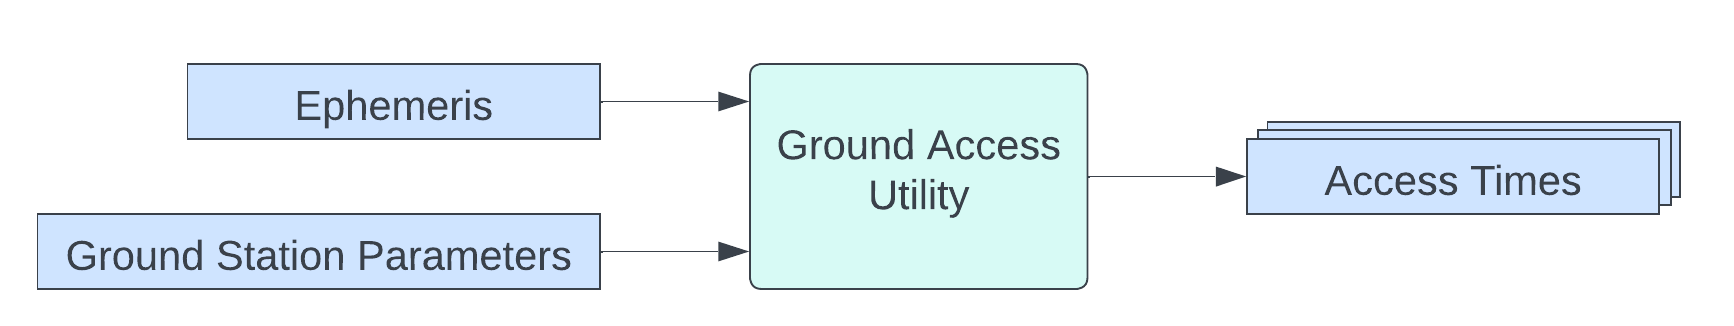
\includegraphics[width=0.7\textwidth]{ATU-1.png} 
    \caption{Input Output Diagram for Ground Access Utilitiy}
    \label{fig:atu-1} 
\end{figure}

So, from a satellite ephemeris and some ground station information, the access
time utilities will generate a list of Access Times. That is, the \textit{time}
of an access and the \textit{type} (access enter or access leave) of an access
will be specified. This is illustrated in Figure~\ref{fig:atu-1}.

\subsection {Swath Utility}

\begin{figure}
    \centering
    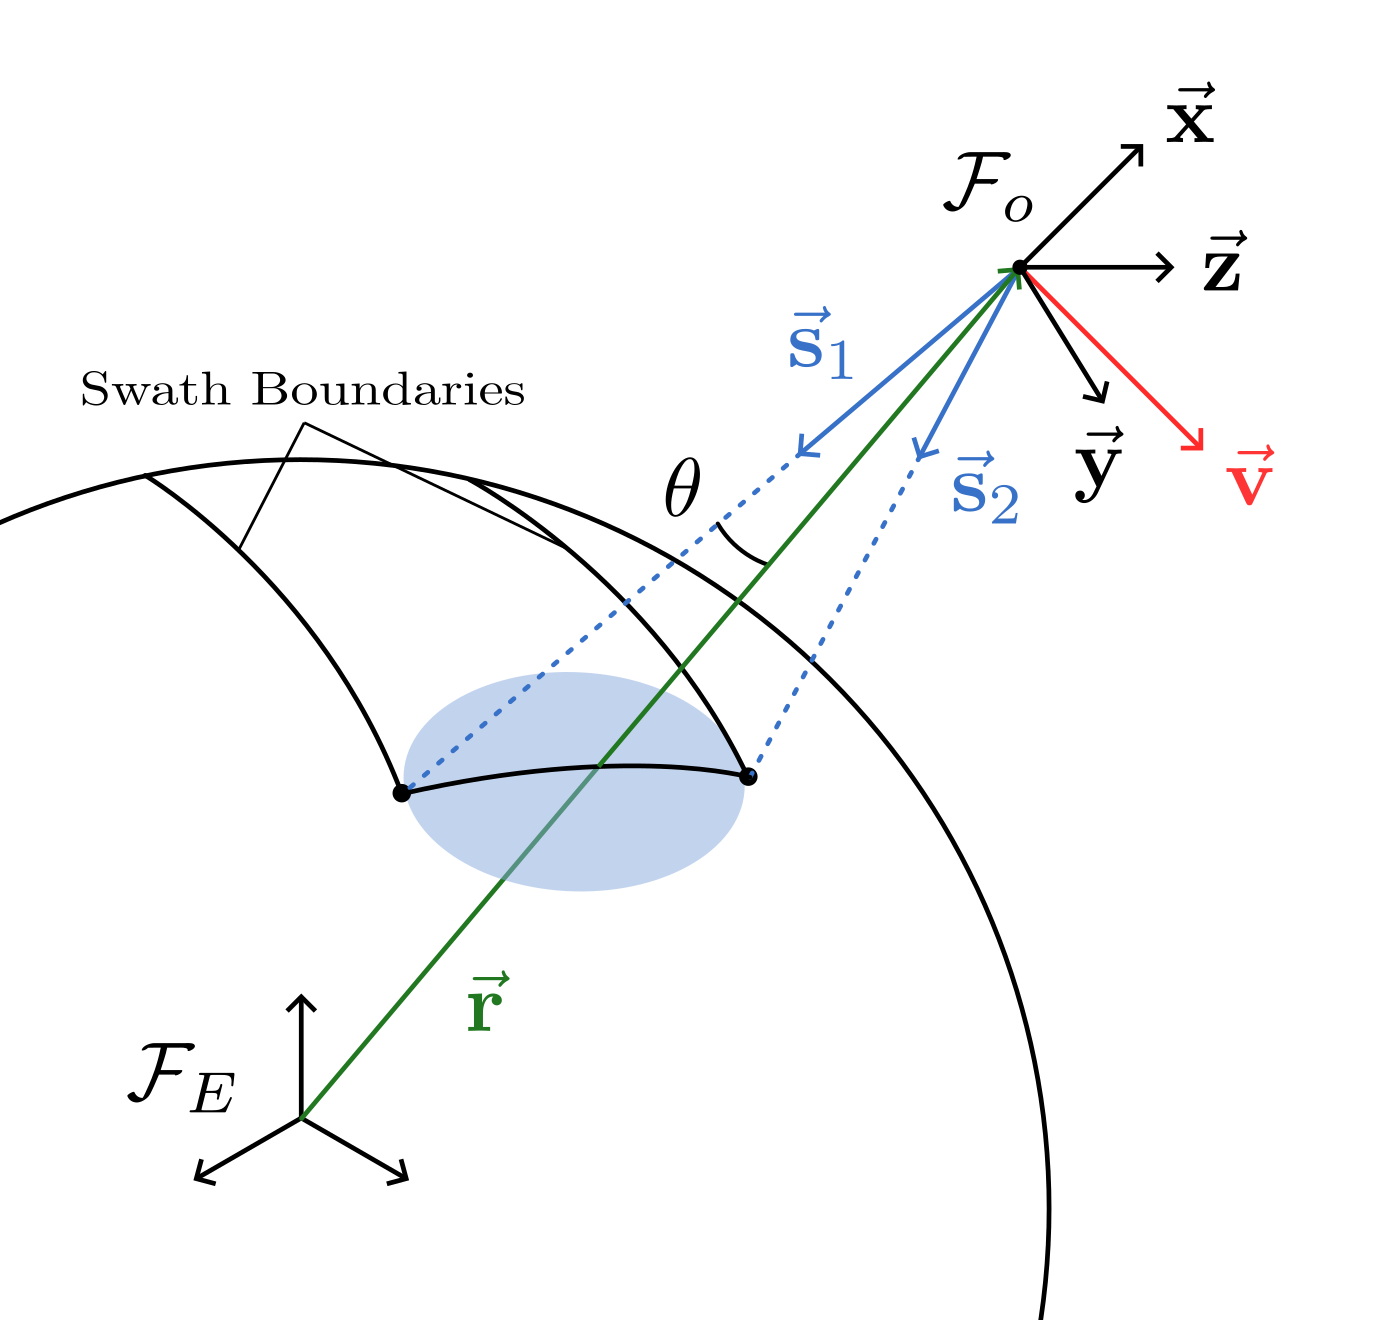
\includegraphics[width=0.5\textwidth]{Swath Bound.png} 
    \caption{Access Swath Boundary Calculation}
    \label{fig:swath-bound} 
\end{figure}

As discussed in the Terminology section, the concept of an access swath is
defined as a time-series of access regions as a satellite orbits the Earth.
Within \gls{pops}, a swath is represented through a closed curve that describes
the boundary of the cumulative footprint/access region of a sensor’s
\gls{fov}/\gls{for} over a time interval. The process for calculating a swath
boundary from an input ephemeris is described here.  

\newcommand{\Fo}{$\vec{\mathcal{F}}_o$} 
\newcommand{\Fe}{$\vec{\mathcal{F}}_E$}

Let us first define the orbital reference frame of the satellite, \Fo, with
respect to an \gls{ecef} fixed coordinate system, \Fe,  Then, let us take the
satellites position, $\sev{r}$, and velocity, $\sev{v}$, with respect to \Fe.
These two vectors are given for a single epoch in an ephemeris file.  \Fo ~is
then defined as $ \vec{\mathcal{F}}_o = \left[ \sev{x}, \, \sev{y}, \, \sev{z}
\, \right]^T$, where:

\begin{equation} 
    \sev{x} = \frac{\sev{r}}{\norm{\sev{r}}}, 
    \quad 
    \sev{z} = \frac{\sev{r}\times\sev{v}}{\norm{\sev{r}\times\sev{v}}}
\end{equation}

And lastly $\sev{y} = \sev{z} \times \sev{x}$ to form an orthonormal set. We
shall then take two vectors, $\sesv{s}{1}$ and $\sesv{s}{2}$, that form the
boundary of our conical FOR and lie within the x-z plane of \Fo,  These are
defined as,

\begin{align}
    \sesv{s}{1} &= \vec{\mathcal{F}}_o^T \left[ \, -\cos\theta, \quad 0, \quad -\sin\theta \right]^T \\
    \sesv{s}{2} &= \vec{\mathcal{F}}_o^T \left[ \, -\cos\theta, \quad 0, \quad \sin\theta \right]^T
\end{align}

Where $\theta$ is the half-angle of the satellite’s \gls{for}. These vectors
are then transformed to \Fe~and the points where they intersect the Earth’s
service are the swath’s bounds for that time instant. If this calculation is
performed multiple times and the boundary points are connected, two lines are
formed on the Earth’s surface. These lines are the satellite’s swath boundary
for that time range.  This process is illustrated in
Figure~\ref{fig:swath-bound}.

%Using the same process, we may also find the ground track of the satellite by
%using the nadir vector, $\sesv{s}{n}$, which is defined as:
%
%\begin{align}
%    \sesv{s}{n} &= \vec{\mathcal{F}}_o^T \left[ 1, \quad 0, \quad 0 \right]^T
%\end{align}

\newcommand{\Cx}[1]{\ses{C}{x}\!\!\left(#1 \right)}

Lastly, we may also approximate the access region for each timestep. To do so,
we can take an off angle vector, $\sesv{s}{1}$, and rotate it around the
x-axis. Where the vector intersects the Earth's surface will be a boundary
point of the access region. For $N$ boundary points, we must rotate the vector
$N$ times. Let us first define a rotation matrix about the x-axis of \Fo~for
some angle, $\phi$:

\begin{equation}
    \Cx{\phi} = 
    \left[
	\begin{array}{ccc}
	1  & 0 & 0   \\
	0 & \cos\phi  & -\sin\phi   \\
	0 & \sin\phi  & \cos\phi
    \end{array}
    \right]
\end{equation}

We may then generate the set of vectors, $S$, that describe the \gls{for} for
that time instant:

\begin{equation}
    S = \left\{ \Cx{2\pi/n} \sesv{s}{1} \, \vert \, n = 1, 2, \ldots N \right\}
\end{equation}
Typically, access regions are described with 8 points but more can be added if
necessary. 


\begin{figure}[h]
    \centering
    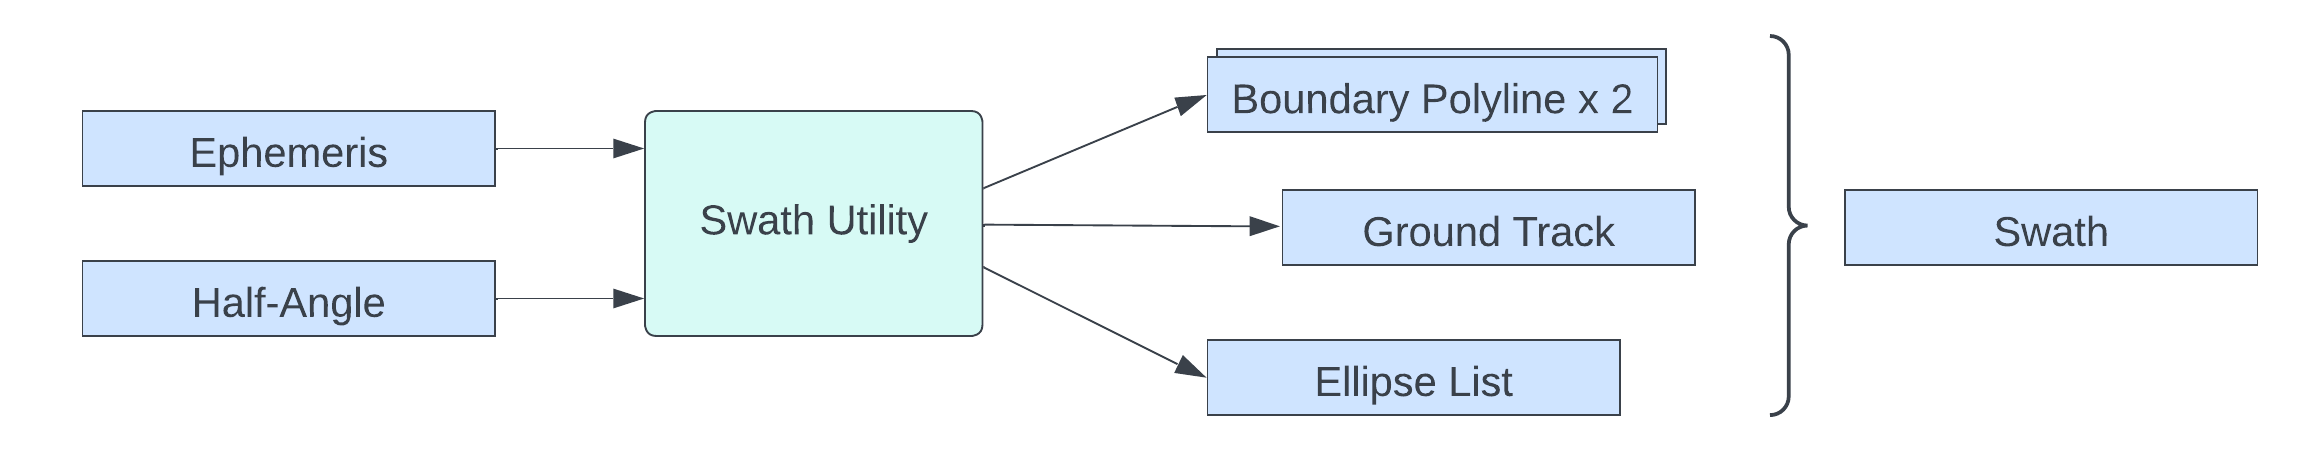
\includegraphics[width=0.7\textwidth]{ATU-2.png} 
    \caption{Input Output Diagram for Swath Utility}
    \label{fig:atu-2} 
\end{figure}

In summary, for every ephemeris point, a swath boundary, a ground track, and a
list of ellipses (access regions) are calculated. This can be seen in
Figure~\ref{fig:atu-2}


\subsection{Swath Intersection Utility}

Swath intersection is an important operation for determining what part of a
specified region is observable by a satellite sensor during some time interval.
Regions are polygons on the Earth’s surface whose vertices are oriented
counter-clockwise. The edge between two consecutive vertices is the great
ellipse arc connecting both points. Swaths are also approximated as polygons
provided that the timestep is small enough. The edge between two swath boundary
points being a great ellipse arc is assumed to be a sufficient approximation.

Polygon clipping techniques are used to find the area of intersection between a
swath and a polygon. First, the swath and polygon vertices are transformed into
2D coordinates. The 2D projection used involves defining a plane that is
tangent to some point on the Earth’s surface.  To project a point on the
Earth’s surface to this plane, a vector is drawn from the centre of the Earth
towards the point (its \gls{ecef} coordinates), and the vector is extended
towards the point of intersection of the plane. This type of projection is
commonly known as the Gnomonic projection; its advantage with respect to the
polygon clipping operation is that great ellipse arcs are projected as straight
lines.  This means classical 2D polygon clipping techniques can be applied to
polygons drawn on the Earth’s surface. So long as the swath and polygon occupy
one hemisphere of the Earth’s surface, the projection will accurately represent
the points of intersection of the swath and polygon, and any polygon clipping
technique can be applied.


\begin{figure}[h]
    \centering
    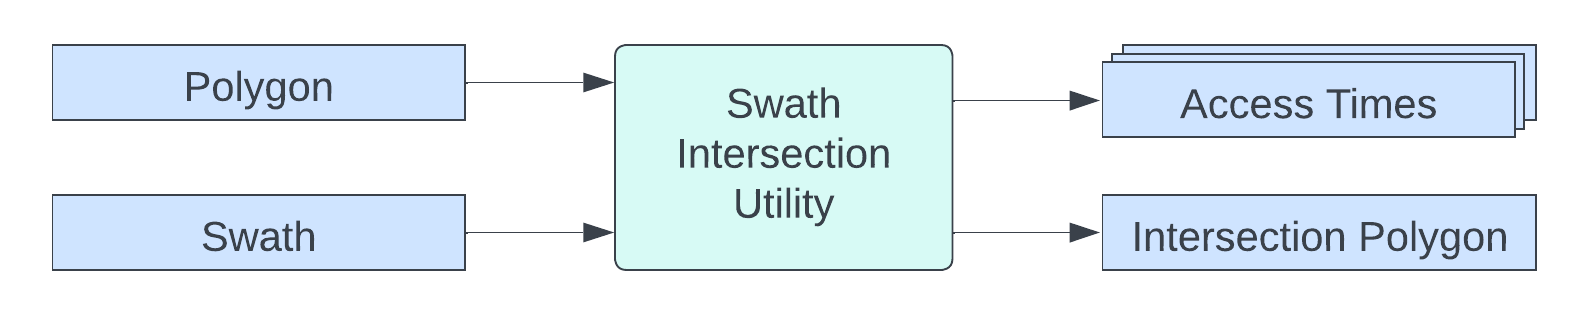
\includegraphics[width=0.7\textwidth]{ATU-3.png} 
    \caption{Input Output Diagram for Swath Intersection Utility}
    \label{fig:atu-3} 
\end{figure}

So given some swath data, specifically the swath boundaries and ellipse list,
the Swath Intersect Utility will return a list of access times and an
intersection polygon between the swath and the polygon. This is illustrated in
Figure~\ref{fig:atu-3}

%% ======================================================================== %%
%%			    Mission Model
%% ======================================================================== %%

\section{Mission Model}
 
The Mission Model service is the service that contains the main logic for most
of \gls{pops}'s functionality and front-end \gls{gui}. When a user interacts
with \gls{pops}, they are interacting with the Mission Model service. As such,
it is quite large and has a number of responsibilities. Some of them are:

\begin{outline} 
    \1 Database management,
    \1 Displaying an interactable front-End User Interface,
    \1 Earth Visualization,
    \1 Plan Configuration, and
    \1 Scheduling.
\end{outline}


\begin{figure}[h]
    \centering
    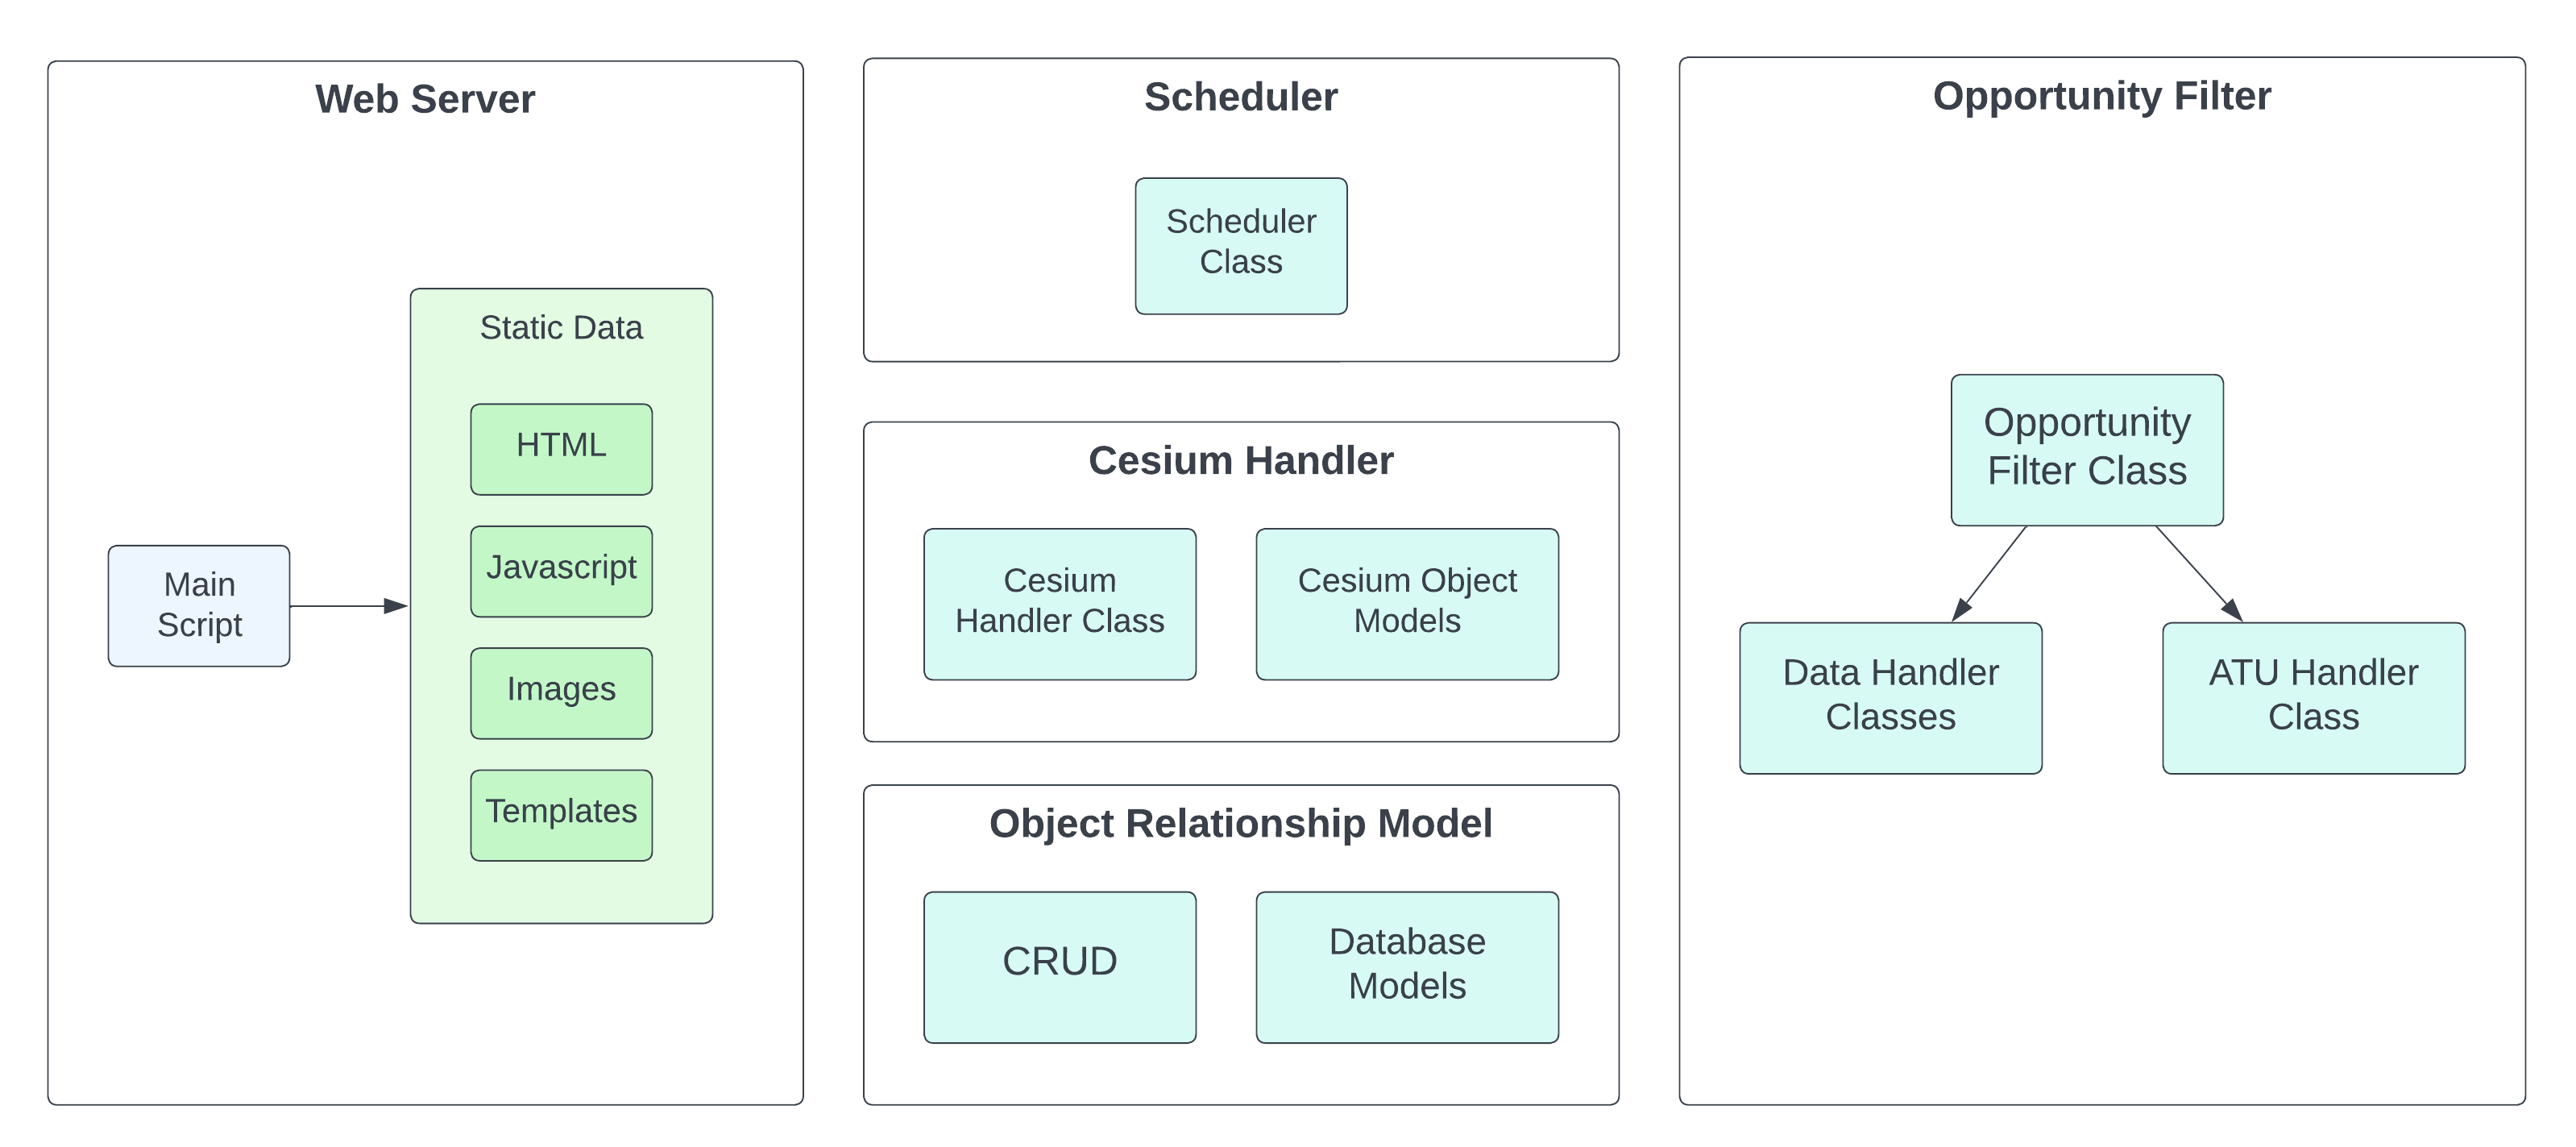
\includegraphics[width=0.7\textwidth]{Mission Model.png} 
    \caption{High Level Structure of Mission Model Service}
    \label{fig:mission_model} 
\end{figure}

A high-level overview of the Mission Model service can be seen in
Figure~\ref{fig:mission_model}. There are many components but this thesis will
go through them one by one.

\subsection{Main} 

The main Python script acts as the base for the entire Mission Model service.
Its purpose is, among other things, to: set up the web server, load environment
variables, instantiate the handler classes, and associate API calls with their
callback functions. Setting up the web server is the same as with any other
service. The environment variables range from server metadata to addresses of
other containers. There are a number of utility classes that handle various
aspects of \gls{pops}. These are the: scheduler, \gls{atu} handler, data
handler, and opportunity filter classes. They will be discussed in the
following sections.  The most important part of the main service is defining
API calls. If a user wishes to interact with \gls{pops}, they must enter a link
on the their browser, that information is then sent to the web server, and a
callback function in the Mission Model service is called. It is the Mission
Models responsibility to consolidate information, whether that be from the
database, through HTML templates, or new information that must be calculated.
The Mission Model service does very few actual calculations, its only purpose
is to organize information and call functions as necessary to serve a request.
Currently, the main service is large and difficult to navigate because of its
size. In the future, it will be refactored to a number of sub-scripts that
handle specific functionality in the service.

\subsection{Object Relationship Mapping}\label{sec:orm}

The Database is its own service but the Mission Model is currently the only
service that interacts with it. It does so by using an \gls{orm}. An \gls{orm}
is a method of modeling a relational database through an object-oriented
language. For \gls{pops}'s purposes, the \gls{orm} serves two functions, it
describes how the data is being stored in the database and it describes how the
database can be interacted with the programmatically. \gls{pops} uses an
open-source \gls{orm} library. It handles the low-level functionality and
allows a developer to focus on what is unique about \gls{pops} rather than
databases in general. For example, there is no need to develop our own methods
of formulating \gls{sql} queries or parsing the output data once it is
retrieved. This has already been implemented many times over in a multitude of
open-source libraries. 

To set up the \gls{orm} for \gls{pops} we need at least two scrips, a models
file and a \gls{crud} file. The models file defines explicitly how tables are
laid out in the database through Python classes. Information such as: what
tables there are, what columns are in each table, what keys are included with a
table, and what relationships there are between tables. If a change is made to
the database, it must be reflected in the models file and vice-versa.  The
\gls{crud} file, as its name suggests, allows us to interact the database.  It
is a library of functions that allows a developer to formulate \gls{sql}
queries at a high level with Python syntax. The \gls{crud} file also relies on
the classes from the models file to refer to tables. For example, if we wished
to retrieve a satellite with a particular id from the \texttt{Satellites}
table, we would create a new function in the crud file with a descriptive name
such as \texttt{get\_satellite\_by\_id(sat\_id)}. Within this function we would
construct a query that searches the \texttt{Satellites} table for a row whose
id column, \texttt{Satellites.id}, matches the input id, \texttt{sat\_id}. The
\gls{orm} gives a developer a great deal of flexibility when formulating
queries or inputting data and makes interacting with the database easy to
understand and easy to expand.


\subsection{Static Data}

For the webserver to function there is a large amount of static data that must
be stored on the server and that must be retrieved when necessary. This may be
\gls{html} files, \gls{html} templates, JavaScript files, \gls{css}
stylesheets, and images.

Webpages are not generated completely programmatically. Either the \gls{html}
for these pages are written in advance and loaded directly upon being requested
or, they are assembled from HTML templates and configured depending on input
parameters given by the user or by what data is available at that time. Writing
out the HTML for a webpage in its entirety is acceptable for situations where
nothing changes on the webpage and everything should be left as is. This is the
case for high-level menus and settings pages. If anything else is required,
\gls{html} templates should be used. HTML templates allow for a great deal of
configurability when loading webpages. They can range from simple text
replacement to loading other templates. Some template engines even allow for
some programmatic features within the template itself such as looping, if/else
statements, or even custom functions.

Generally, as a design decision, as much of the underlying logic for \gls{pops}
has been limited to Python. The main reason for this is to consolidate the
logic to one language. Unfortunately for web development, JavaScript and
\gls{css} are unavoidable and must be used. When they are used they can be
added directly to an HTML document or template but this is generally not the
best way. Having different scripts or different styles placed haphazardly in
the codebase gets messy quickly and may lead to code duplication or even
conflicts. To address this, JavaScript and \gls{css} files are stored
separately and then statically referenced in the \gls{html} file they apply to.
By consolidating these files, it is much easier to organize and reference them
as necessary. 


\subsection{Data Handlers}\label{sec:data_handler}

For \gls{pops}, there is a great deal of data and there are many different ways
that the data can be formatted in. In an attempt to generalize the data and
make it easier for a developer to work with, several Data Handler classes have
been created to handle data format conversions and to provide helper functions.
The differences in data formats can be as simple as differences in what keys
are used in dictionaries of key-value pairs. For example, the Propagator
service uses the key \texttt{`position'} and the \glspl{atu} use the key
\texttt{`pos'}.  This is a small discrepancy and if all the differences were
this simple, then some standard data format would just be adopted.
Unfortunately, there are larger differences that require conversion.  When
describing lists of points there are currently 3 different formats. The
Propagator service generates a list of points, $P_1$, as a list of the x, y,
and z components for all $N$ points. 

\begin{align*}
    P_1 &= [\se{x}, \se{y}, \se{z}] 
\end{align*}
where
\begin{align*}
    \se{x} &= [x_0, x_1, x_2, \ldots, x_N],  \\
    \se{y} &= [y_0, y_1, y_2, \ldots, y_N],  \\
    \se{z} &= [z_0, z_1, z_2, \ldots, z_N]
\end{align*}

To describe swath boundaries as lists of points, $P_2$, the \gls{atu} service
uses a dictionary of key-value pairs. There is one string key for each
component (\texttt{`x'}, \texttt{`y'}, and \texttt{`z'}) and the value for each
is the list of components for all $N$ points. 

\begin{equation*}
    P_2 = 
    \left\{
    \begin{aligned}
	\texttt{`x'}&: [x_0, x_1, x_2, \ldots, x_N],  \\
	\texttt{`y'}&: [y_0, y_1, y_2, \ldots, y_N],  \\
	\texttt{`z'}&: [z_0, z_1, z_2, \ldots, z_N]
    \end{aligned}
    \right.
\end{equation*}

Lastly, the graphical Earth Visualization tool, Cesium, expects lists of
points, $P_3$, to be a single list, where the components of each point are
ordered one after the other.

\begin{equation*}
    P_3 = \left[ x_0, y_0, z_0, x_1, y_1, z_1, \ldots x_N, y_N, z_N \right]
\end{equation*}

All of these formats contain the same information but organized in different
ways.  A developer should not have to write conversions whenever they wish to
use a data type.  They should only have to worry about the data itself and not
how it needs to conform with whatever format. It is for this reason we must
consolidate these conversions in separate data handler classes.  Of course,
there is much more data and many more data formats that must be supported, but
these three examples are sufficient to give the reader an idea about the
nuances involved. There are many Data Handler classes but the following are
some of the larger more important ones.


\subsubsection{Ephemeris Data Handler}

Ephemerides are the most important collections of data as they are used as a
basis to calculate most other data. As such, they are referenced many times and
have a number of different formats. There are four different areas where
Ephemerides are referenced: the Propagator service, the \gls{atu} service, the
Cesium Viewer, and the Database. An Ephemeris object contains some of the
following information:

\begin{description}

    \item[Epoch] An ISO 8601 Datetime string in UTC specifies the reference
	time for the ephemeris data.

    \item[Seconds] An array of float values that specify the offset from the
	epoch.

    \item[Position] Position vectors of the satellite. Each corresponds to a
	seconds offset.

    \item[Velocity] Velocity vectors of the satellite. 

    \item[Pass Index] For each ephemeris point, the pass index is specified. 

\end{description}


An Ephemeris object can either be created by sending a request to the
Propagator service or it can be loaded from the Database. For the case where we
generate a new ephemeris from the Propagator service, the Ephemeris class
handles communication with the Propagation service and directly saves the
outputted ephemeris data into a private variable. The propagator ephemeris data
format serves as the base format from which we can convert to other formats as
necessary. For example, there are member functions that take the saved
ephemeris data and converts it into the format expected by the \glspl{atu} or
into a format expected by Cesium. Alternatively, if an ephemeris is loaded from
the database, each row must be sorted, processed, and converted to the base
format. 

In some scenarios we do not wish to work with an entire Ephemeris for a large
scenario, rather we may wish to only consider a subset of a larger Ephemeris
object. When we take a subset of a larger Ephemeris, we refer to this process
as `constraining' the Ephemeris. For this, a helper function has been added
which accepts a time range that lies within the time range the Ephemeris object
is defined for. This helper function then generates a new Ephemeris object
which only contains the ephemeris data that lies in the desired time range.  

\subsubsection{Swath Data Handler}

The Swath Data Handler classes behaves very similarly to the Ephemeris Data
handler. It too must have data conversion methods for the \glspl{atu}, for
storage and retrieval from the database, and for loading into Cesium. It also
has a helper function that constrains the Swath object to a specified time
range. 

It should be noted that at this level, there is no distinction between an
access swath and a ground swath. Both are generated in the same way, stored in
the same way, and displayed in the same way. Whether they are defined based on
a \gls{fov} or \gls{for} is immaterial and not relevant in this context. 

The data a Swath object stores is similar to an Ephemeris object. It has an
epoch and a seconds array. These match the epoch and seconds array of the
Ephemeris object the Swath object was generated from. Swath objects may also be
constrained in the same way Ephemeris objects may be. In summary, a swath
object contains the following data:

\begin{description} 

    \item[FOV/FOR] For reference the FOV or FOR angle is stored along with the
	swath data.

    \item[OFF-1/2] These are the boundary polylines of the Swath object. They
	are stored as lists of points.

    \item[Ground Track] For display purposes, it may be useful to display the
	ground track of the satellite generating the Swath Object so this
	information is stored as a list of points.

    \item[Ellipse List] Each timestep in a Swath Object is also given an
	Ellipse which represents the footprint/access region. 

\end{description}


\subsubsection{Polygon Data Handler}

The Polygon Data Handler is the last data handler class of note. It is used to
represent area target \glspl{aoi} or intersection polygons. The core data a
Polygon object contains is simply just a single list of points.  As with the
Ephemeris and Swath data handlers, there is a small sweet of data format
conversions.  But, for the Polygon Data Handler, much of the functionality lies
in its utility functions.

The first utility function is simple; it merely transforms all of the points in
the Polygon from \acrfull{ecef} Cartesian-xyz coordinates to
Latitude-Longitude-Altitude coordinates and vice-versa.  Generally, with other
objects such as Ephemeris objects or Swath objects, their underlying data will
never be explicitly displayed to the user. For this reason, points in those
objects can be left as Cartesian coordinates. But, when a user creates a
Polygon object or if the coordinates of the vertices need to be displayed to
the user, Latitude and Longitude is much more human readable than Cartesian
coordinates. 

Early on in development, there were some restrictions placed on the types of
polygons that the \glspl{atu} could accept. One restriction was that polygons
must be convex. That is for the set of all points that lie within a polygon,
there do not exist two points such that if a line is drawn between the points,
that line intersects with an edge of the polygon. At first, it seemed as though
this only limited the types of area-targets that could be specified. Through
developing the opportunity filter class, there arose some scenarios where
concave polygons were generated that needed to be inputted into the
\glspl{atu}. For this reason, a simple algorithm was implemented that removes
vertices to force a polygon to be convex.  

%The implementation for this is
%discussed in Algorithm~\ref{alg:force-convex}.  Thankfully, this restriction
%has been lifted but the implementation is interesting nonetheless.

Another restriction placed on polygons is that their vertices must be ordered
counter-clockwise (the motivation for this is discussed in
Section~\ref{sec:cesium-models}). If a polygon is ordered in a different way,
this may lead to garbled results from the \glspl{atu} or Cesium viewer. If
necessary, when generating a Polygon object and a developer suspects that the
source data may be un-ordered, they may set an option to \textit{force} a
polygon to be counter-clockwise. Re-ordering is not always perfect, though, and
that is why this is an option and not always done. 

%The implementation for this can be found in Algorithm~\ref{alg:ccw}.


\subsubsection{Other Data Handlers}

There are a number of other data handler classes that are used but don't have
as much notable functionality. Some of these are:

\begin{itemize} 
    
    \item Access Times Data Handler
    \item Ground Station Data Handler
    \item Sensor Data Handler

\end{itemize}

%For the Access Times Data Handler, there exists one utility function. There are
%some situations where a developer may need to determine what access times, if
%any, lie within some defined period of time. For this the Single Access
%Intersection algorithm was developed which is discussed in
%Algorithm~\ref{alg:contains}.


\subsection{Access Time Utilities Handler}

In order to abstract the communication between the Mission Model service and
the \gls{atu} service, an \gls{atu} handler class has been developed. Its
purpose is simple, from input data, it sends requests to the \gls{atu}
service and formats the result. A developer shouldn't need to create a POST
request every time they wish to utilize some \gls{atu} functionality. They
may make a mistake and debugging wastes development time. 

Every \gls{api} call provided by the \gls{atu} service has a corresponding
method in the \gls{atu} handler. For ease of use, the inputs and outputs of
each method are Data Handler objects. For example, if a user wishes to perform
polygon intersection with a swath and a polygon, all they must do is pass a
Swath object and Polygon object to the \texttt{polygon\_intersection()} method
and an Access Times object and another Polygon object will be returned. The
purpose of this is to make interacting with the \gls{atu} service as simple as
specifying their high-level inputs and outputs.


\subsection{Opportunity Filter}

The Opportunity Filter class is the most important but also most complex aspect
of the Mission Model service. It is here that the Mission Model actually
searches for potential observation opportunities and implements the filters
discussed in Section~\ref{sec:opp-filtering}. Its purpose is to combine
the functionality of the Data Handler classes and the \gls{atu} Handler class
to make Opportunity Filtering as close as possible to their high-level
summaries. In general, with opportunity filtering, the implementation process
is straightforward and matches well with its high-level description. This is
not always the case though. Let us now revisit the Filters discussed earlier,
and outline how they are actually implemented in \gls{pops}. 

\algnewcommand\algorithmicforeach{\textbf{for each}}
\algdef{S}[FOR]{ForEach}[1]{\algorithmicforeach\ #1\ \algorithmicdo}

\begin{algorithm} 
    \caption{Coarse Imaging Opportunity Filter}
    \label{alg:coarse-imaging} 
    \begin{algorithmic}[1]
	\Function{CoarseImaging}{$E_A$, $g_{AOI}$} 

	    \Let{$S_A$}{\Call{Swath}{$E_A$, $60^\circ$}} \Comment{Coarse Imaging Swath}

	    \Let{$A_{A}$, $G_A$}{\Call{PolygonIntersection}{$S_A$, $g_{AOI}$}} 

	    \Let{$O$}{$[A_{A}, G_A]$} \Comment{List of Opportunities}
	\State \Return $O$, $S_A$
	\EndFunction
    \end{algorithmic}
\end{algorithm}

The implementation of the Coarse Filter can be seen in
Algorithm~\ref{alg:coarse-imaging} and is very close to its high-level
description. The inputs to the filter are the Ephemeris of Sat-A, $E_A$, and
the Area of Interest polygon $g_{AOI}$. First the coarse imaging swath is
generated, $S_A$. Then the swath and \gls{aoi} are passed into the Polygon
Intersection Utility which return a list of access times, $A_{A}$, and a list
of intersection polygons, $G_A$. Note that the length of $A_{A}$ and $G_A$
are the same since you cannot have an intersection polygon without an access.
Given this property, the list of opportunities, $O$, is only the combination of
$A_{A}$ and $G_A$. Finally, the list of opportunities is returned along with
the coarse imaging swath. 

Some details of the polygon filtering process have been omitted for clarity.
That being, the insertion of all the data into the database. How opportunities
are actually stored, as mention in the Section~\ref{sec:database}, is that
first, the search data is generated, then it loaded into the database, and
finally each opportunity is a list of database ID's corresponding to each
search element. The purpose of this is to not duplicate data and to also allow
an opportunity to be defined with as many search elements as is desired by a
developer.


\begin{algorithm} 
    \caption{Tip-and-Cue Imaging Filter}
    \label{alg:tip-and-cue} 
    \begin{algorithmic}[1] 
	\Require{$E_A$ and $E_B$ must be defined for the same time range and time step.}
	\Function{TipAndCueImaging}{$E_A$, $E_B$, $g_{AOI}$, $L_G$} 

	    \Let{$S_A$}{\Call{Swath}{$E_A$, $60^\circ$}} \Comment{Tip Swath}
	    \Let{$S_B$}{\Call{Swath}{$E_B$, $20^\circ$}} \Comment{Cue Swath}

	    \Let{$A_{G,A}$}{\Call{GroundAccess}{$E_A$, $L_G$}} \Comment{Calculate Ground Accesses}
	    \Let{$A_{G,B}$}{\Call{GroundAccess}{$E_B$, $L_G$}}

	    \Let{$A_{A}$, \_}{\Call{PolygonIntersection}{$S_A$, $g_{AOI}$}} 

	    \ForEach{$a_A$ in $A_{A}$}

		\Let{\_, $g_A$}{\Call{PolygonIntersection}{$S_A(a_A)$, $g_{AOI}$}} 
		\Comment{Constrain Swath to access}

		\Let{$p$}{\Call{Pass}{$E_A$, $a_A$}} \Comment{Get pass that contains access}

		\Let{$a_B$, $g_{A \wedge B}$}{\Call{PolygonIntersection}{$S_B(p')$, $g_{A}$}} 
		\Comment{Constrain Swath to next pass}

		\If{ $\exists \alpha \in A_{G,A}, \exists \beta \in{A_{G,B}}, (a_A < \alpha, \beta < a_B) $}
		    \Let{$O$}{$O + (a_A, a_B, g_{A \wedge B})$}
		\EndIf

	    \EndFor

	\State \Return $O$, $S_A$, $S_B$
	\EndFunction
    \end{algorithmic}
\end{algorithm}

Tip-and-Cue Filtering can be seen in Algorithm~\ref{alg:tip-and-cue}. The main
components of the filter are still there but some modifications have been made
as part of the implementation and to speed up processing. Let us walk through
the filter. As expected, the inputs to the filter are merely the ephemerides
for both Sat-A and Sat-B, $E_A$ and $E_B$, and the \gls{aoi}, $g_{AOI}$. In
addition to these, we also include a list of ground stations that are available
for this mode, $L_G$. From the ephemerides the tip and cue swaths are
generated, $S_A$ and $S_B$.  Using the Ground Access Utility we can generate
lists of ground access times for Sat-A and Sat-B, $A_{G,A}$ and $A_{G,B}$ for
every ground station provided. 

After this, instead of calculating all of intersection polygons for the tip
swath and the \gls{aoi}, only the list of access times are recorded, $A_A$.
This has two purposes.  First, it is faster to just calculate the access times
for the Intersection Polygon Utility. Second, this gives us a list of access
times that can be iterated over to find opportunities. The significance of this
is that there may exist \glspl{aoi} where Sat-A has multiple accesses within a
single pass. By iterating over each access we create an opportunity for every
access in a pass.  The alternative would be to iterate over every pass. This
method would either require taking only the first access in the tip pass as an
opportunity or specialized logic would be needed that would over complicate the
filter.

With an access list for Sat-A, we can iterate over every individual access,
$a_A$. The first operation in each iteration is to calculate the Intersection
Polygon of Sat-A and the \gls{aoi} during that access. Note the notation used,
$S_A(a_A)$ indicates that the swath is constrained to only the time range
within the parentheses. Next we find the pass, $p$, the access lies in.  This
is done with a built-in helper function in the Ephemeris Data Handler Class.
From this pass index we can constrain the Cue swath to only the next pass and perform
Polygon Intersection with it and the intersection polygon from the previous
step. This outputs the access time for Sat-B, $a_B$ and the Intersection
Polygon for Sat-A, Sat-B, and the \gls{aoi}, $g_{A \wedge B}$. Before adding an
opportunity, we must check if suitable ground station contacts exist in between
Sat-A's access and Sat-B's access. If this is the case Sat-A's access, Sat-B's
access, and the intersection polygon are then appended to the list of
opportunities. Otherwise the opportunity is discarded. This process is then
repeated for each of Sat-A's access times.

From this process, some edge cases have been omitted. That being, at the
beginning and end of a scenario, we cannot generate any opportunities because
there would be no corresponding tip or cue pass respectively. Also, another
edge case would be where there are no accesses for Sat-A and Sat-B in a single
pass. Similarly, the process of adding the search data to the database is also
omitted.


\subsection{3D Earth Visualization}

One of the required components of \gls{pops} is a graphical 3D Earth viewer.
It goes without saying that having a spatial understanding of a mission is
absolutely necessary when performing mission planning. Only so much information
can be imparted through text.


To support this functionality, \gls{pops} makes use of the open-source CesiumJS
library. CesiumJS can display time-dynamic, geospatial information on a
webpage. CesiumJS itself is free to use and provides all of the core
functionality that is necessary for \gls{pops}. There also exists a proprietary
library, CesiumION, which provides out-of-the-box 3D terrain data and
proprietary Earth imagery. Thankfully this kind of information is superfluous
for orbit operations planning. At most, all that is needed is a rough
understanding of the Earth's geography and that is sufficient. For this reason,
\gls{pops} does not provide terrain information and uses a free tile map
provider. Since \gls{pops} is only using the free version, we will refer to
CesiumJS as just Cesium for brevity. 

It should be noted that Cesium is only meant to display information to the user
and not intended to be a tool that performs any calculations. All data is generated
through other means and then converted into a format that Cesium can display.
The reason for this is that, since Cesium is such a large tool, it is difficult
to validate in great depth because it is not clear what assumptions are being
made at what level. So, as long as the entities being displayed by Cesium are
qualitatively correct then that is sufficient.

\begin{figure}[h]
    \centering
    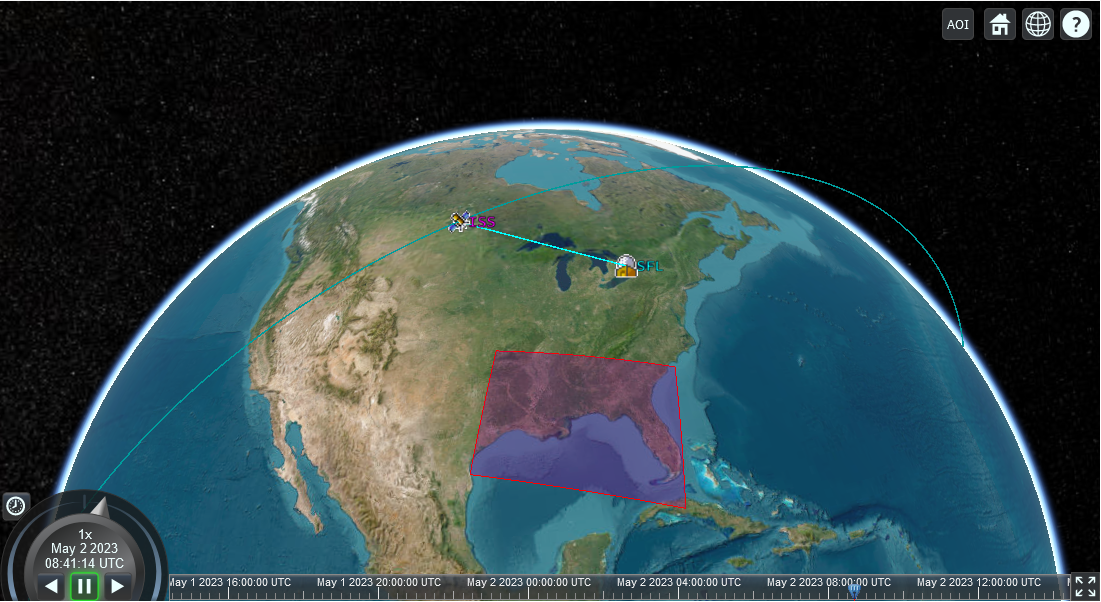
\includegraphics[width=0.9\textwidth]{Cesium_Example_Image.png} 
    \caption{Cesium Example Scenario with Example Entities}
    \label{fig:example_cesium}
\end{figure}

An example scenario generated by \gls{pops} can be seen in
Figure~\ref{fig:example_cesium}. There, a few key elements of a Cesium viewer
are visible. On the bottom, there is a timeline with some controls. A user can
change the time of the scenario as they like and the scenario will update
dynamically. This is very similar to tools such as \gls{stk} so an operator
will be used to working in this way. In the centre the Earth can be seen with
the camera hovering over North America.  The camera can be moved with the mouse
or can be fixed to a particular position and orientation programmatically.
Some entities have been added to the scenario. At the bottom, a polygon has
been drawn on the Earth. A very useful feature of Cesium is that polygons can
be defined with vertices and edges clamped to the WGS84 Ellipsoid. That is,
vertices are placed on the Ellipsoid and edges are not straight lines but great
ellipse arcs. This saves a great deal of calculations and code that must be
maintained. Above the polygon, can be seen a satellite, the \gls{iss}, and a
ground station, the \gls{sfl}. The ground station is fixed but the satellite
orbits the Earth and changes position as the time changes in the scenario. The
satellite's path is given by the teal line. 

Every object in the Cesium viewer is treated as a single entity. There are two
ways entities may be added, updated, or removed from a Cesium viewer. Either,
through JavaScript, where a developer creates new objects programmatically, or,
through a custom \gls{json} format called \gls{czml}. Though Cesium has an
extensive client-side \gls{api}, \gls{czml} allows the cesium scenario to be
generated from data rather than from custom code. Most of the underlying data
is calculated through Python scripts so it is more appealing to have an
interface that generates \gls{czml} data rather than having additional
JavaScript. Also, by generating \gls{czml}, logic is not split between the
backend Python code and front-end JavaScript. In this way, the Python drives
what is being shown in the Cesium viewer. \gls{czml} also allows for
incrementally streaming data to a client. That is, not all of a scenario needs
to be available immediately once a scenario is loaded. Rather, \gls{czml} data
can be sent in a number of packets, and can be added as they become available.

To set up a viewer, some JavaScript is needed. A placeholder is placed
somewhere in the webpage hosting the viewer then the JavaScript searches for
that placeholder and inserts all of the necessary data to generate the viewer.
Some parameters need to be set for the viewer such as: the imagery provider,
rendering modes, lighting, display options, or toolbar buttons. Once a viewer
is created, it runs until it or the page is changed.  To facilitate
communication between the Cesium viewer and the Python backend, a websocket is
created as they allow for bi-directional communication. 

\subsection{Cesium Models}\label{sec:cesium-models}

Even though we are using Cesium as our 3D Earth visualization tool, a
substantial amount of development must be done to properly configure and manage
what is being shown on the viewer. Before discussing how a Cesium viewer is
managed, it would be useful to first go over what can be displayed currently
with \gls{pops}, the Cesium Models. These model classes are not like the ones
made for \gls{orm}, rather these models have two responsibilities. They must
keep some metadata about a Cesium object and they must contain a method that
generates a valid \gls{czml} packet.  A \gls{uml} diagram that summarizes all
of the currently implemented Cesium models can be seen in
Figure~\ref{fig:cesium_models}. It should be noted that the diagram does not
contain an exhaustive list of all of the member variables for each class;
rather, it contains the most important variables.  Each model contains some
information about the object that does not change once it is created. For
example a satellite object will not change which satellite it references once
it's created. 

\begin{figure} 
    \centering
    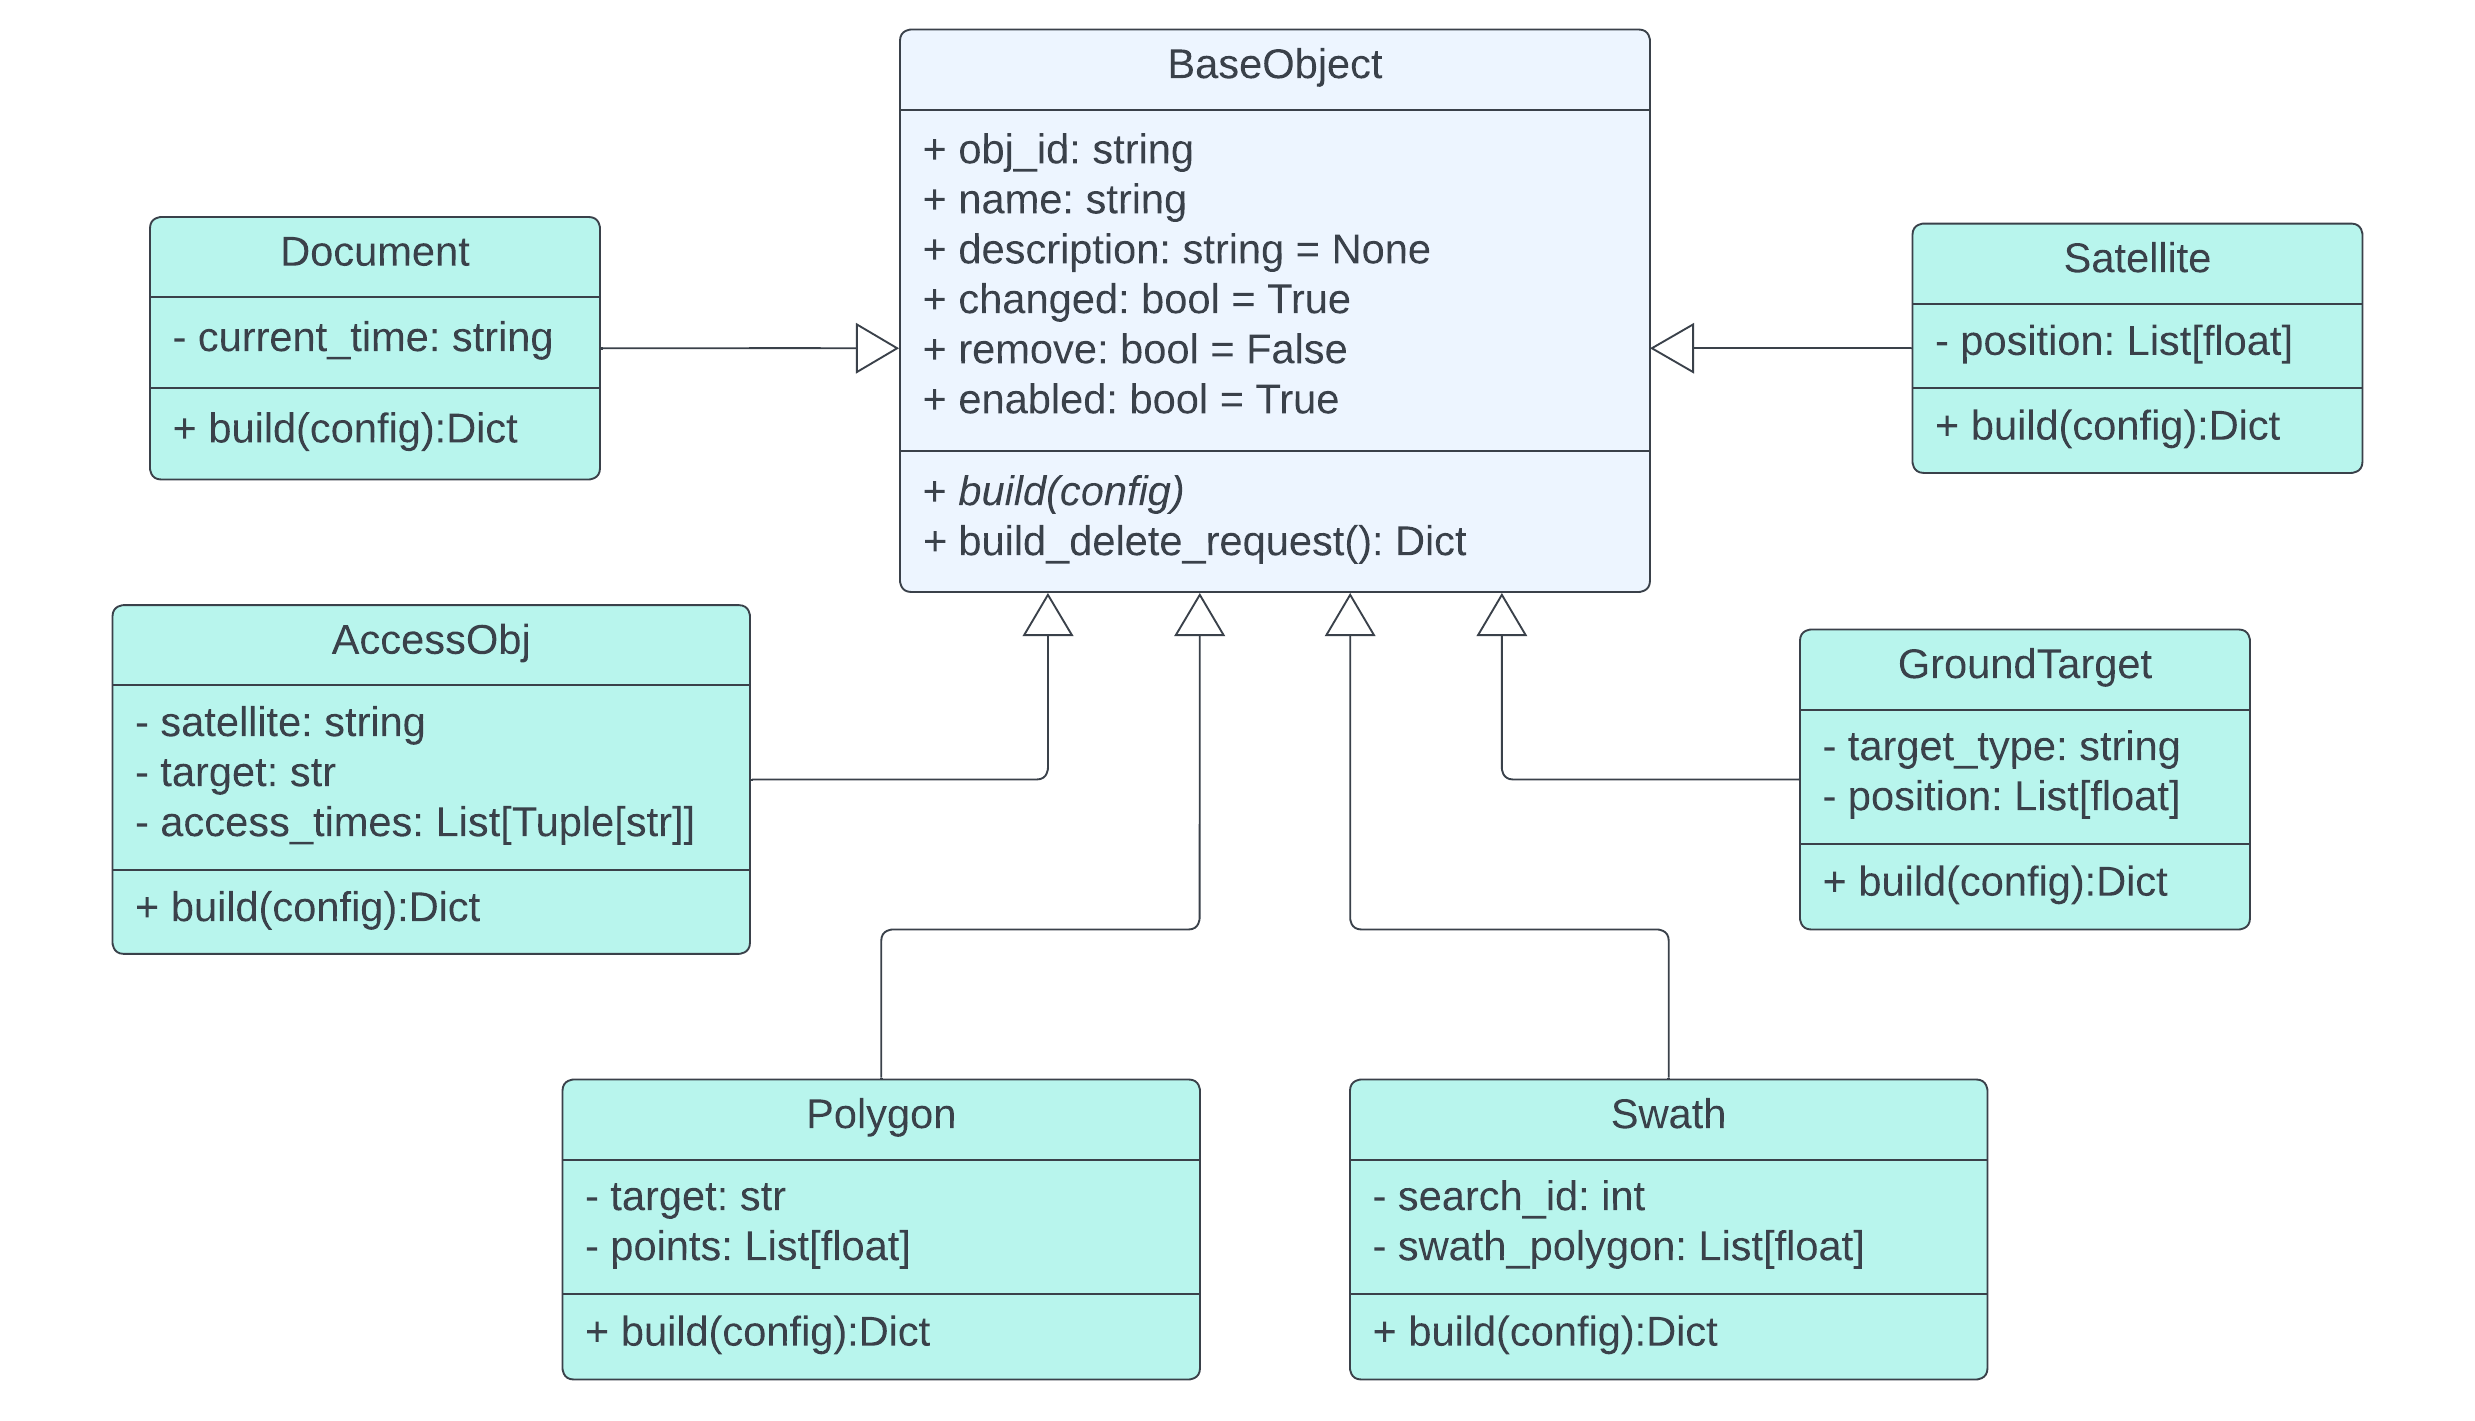
\includegraphics[width=0.9\textwidth]{Cesium_Models.png} 
    \caption{Cesium Models UML} 
    \label{fig:cesium_models} 
\end{figure}

To begin, there is a \texttt{BaseObject} class which serves as a general parent
class to all Cesium objects. It defines member variables that are common to all
objects. Properties such as the object's unique ID, its display name, and its
description. In addition there are three flags that describe the `state' of the
object: \texttt{changed}, \texttt{remove}, and \texttt{enabled}. If the
\texttt{changed} flag is set, this indicates to the Cesium Handler class that a
new \gls{czml} should be generated for that object. By default, every time an
object is created, the \texttt{changed} flag should be set. Once \gls{czml} is
generated and uploaded to the viewer, this flag is reset. If the
\texttt{remove} flag is set, this object should be removed from the Cesium
viewer, and once this is done, the object should be deleted. Lastly,
\texttt{enabled} hides Cesium Entities without unloading them from the viewer.
Each sub-class has its own implementation of the \texttt{build()} method, since
building a \gls{czml} object is unique to that object.
\texttt{build\_delete\_request()} is common to all Cesium objects since the
request only contains the object's ID. The currently supported Cesium models
are as follows:

\begin{description} 

    \item[Document] Each Cesium scenario must have one and only one
	\texttt{Document} object as it specifies general scenario data such as:
	what is the scenario's time range, what is the current time in the
	scenario, or what is the scenario's timestep. Once this object is set
	for a scenario, it does not need to be set again unless the current
	time should be changed.

    \item[Satellite] Satellites are represented through a small \gls{png} image
	called a `billboard'. In the future, 3D models may be used instead but
	images are sufficient for now. A satellite is also given a descriptive
	label that maintains a fixed position with respect to its position. To
	have the satellite move over time within the scenario, an ephemeris
	must be included in the object.  This ephemeris must conform to a
	particular format and this conversion is handled by the Ephemeris data
	handler discussed in Section~\ref{sec:data_handler}.  Lastly, a
	satellite is given a path to visualize to the user, where the satellite
	will be and has been for some period in the future and the past.

    \item[Ground Target] Ground Targets are essentially the same as Satellite
	objects but, in this case, they are given only one position for the
	entirety of the scenario. Ground Targets can be \glspl{aoi}, ground
	stations or any other stationary ground object.

    \item[Access Object] It is useful to display when a satellite has access to
	a ground target. This is accomplished through drawing a line between
	the satellite and the ground target for times where they have access to
	each other. One useful feature of \gls{czml} is that we can reference
	the position of other object by reference to their ID. This saves us
	from having to load a satellite ephemeris into the object to describe
	the position of the satellite. \gls{czml} also allows us to specify
	when an object should or should not be visible by specifying intervals
	of visibility. When an \texttt{Access Object} is created we must pass a
	list of access times such that we may define these intervals in the
	object.

    \item[Polygon] As mentioned earlier, Cesium has the ability to display
	polygons in any number of ways but, for our purposes, we are mainly
	focused on polygons clamped to the Earth's surface. The two instances
	where polygons are currently used for \gls{pops} are for Area Target
	\glspl{aoi} and for intersection polygons. The difference practically
	for these two cases is just in their colour. To draw a polygon in
	Cesium, we must provide it a list of points in Cartesian coordinates or
	in Latitude-Longitude-Altitude coordinates. For the Cartesian
	coordinates, if a point does not directly lie on the WGS84 Ellipsoid,
	Cesium will only draw the closest point on the Ellipsoid. From this
	list of points, Cesium will guess the `inside' of the polygon. Note
	that since we are drawing shapes on an Ellipsoid, the geometry is
	non-Euclidean. The inside of a polygon on a 2D plane is clear for
	polygons that do not self-intersect; it is simply the region that
	is enclosed by all of the sides of the polygon. For an Ellipse any
	point can be enclosed. See an example of this in Figures
	\ref{fig:inside_polygon_1} and \ref{fig:inside_polygon_2}. Both have
	identical polygons where there are 4 vertices on the Ellipsoid and
	their edges are the same. There is now a question of what forms the
	inside of the polygon as this can be the larger area or the smaller
	area. There are a number of ways this can be addressed. One way is to
	specify the points on the polygon in a clockwise or counter clockwise
	order. Then the internal area will be whatever conforms to this
	ordering. Another way would be to specify one or more points that are
	not vertices but rather example points that lie within the polygon. In
	this way the area of the polygon will be the set of points that contain
	the example point. For simplicity, Cesium makes a best guess at what
	the inside of a polygon is by selecting the inside with the smaller
	area. This is sufficient for smaller polygons but for larger or more
	complicated polygons where the intended area is greater than one half
	hemisphere, determining the inside of a polygon no longer becomes clear
	and the viewer displays a garbled result. Alternatively, if there is a
	polygon which intersects itself, Cesium also becomes confused. In these
	scenarios, a large polygon must be sub-divided into sections that
	Cesium can process.

\begin{figure}
    \begin{minipage}[c]{0.45\textwidth}
	\centering
	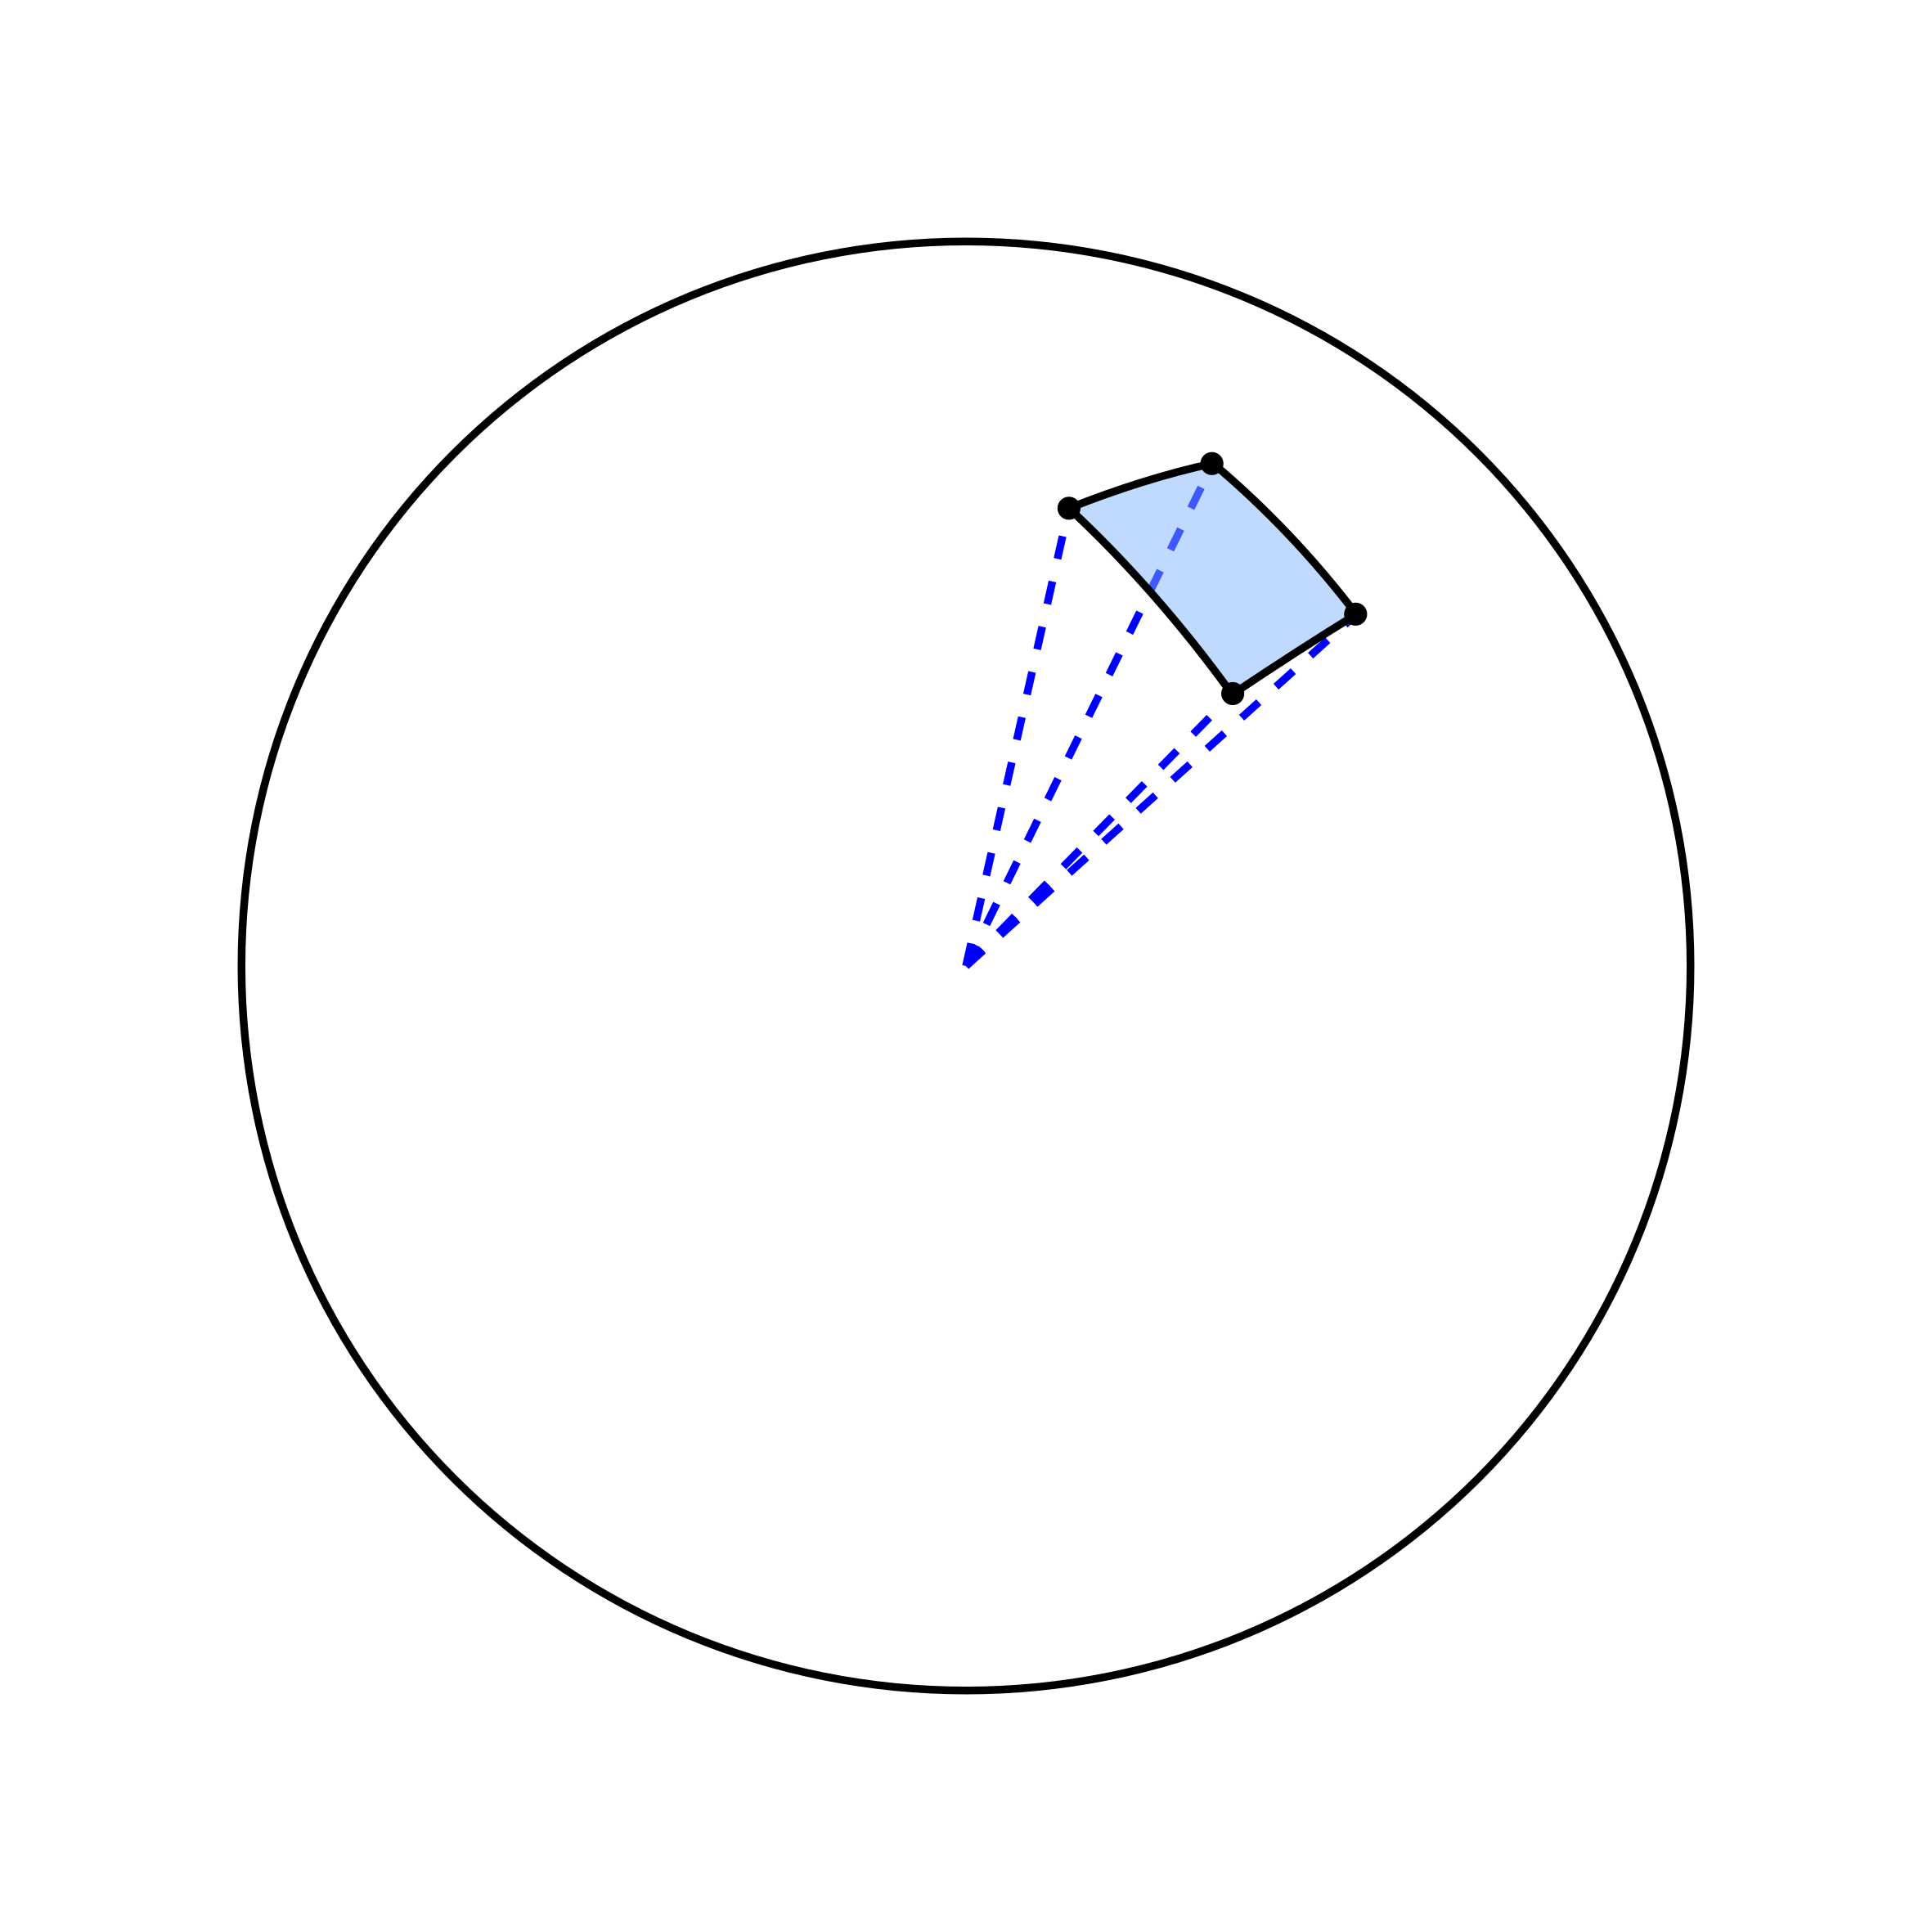
\includegraphics[width=1\textwidth]{inside-outside-2.png} 
	\caption{Smaller Area}
	\label{fig:inside_polygon_1}
    \end{minipage}
    \hfill
    \begin{minipage}[c]{0.45\textwidth}
	\centering
	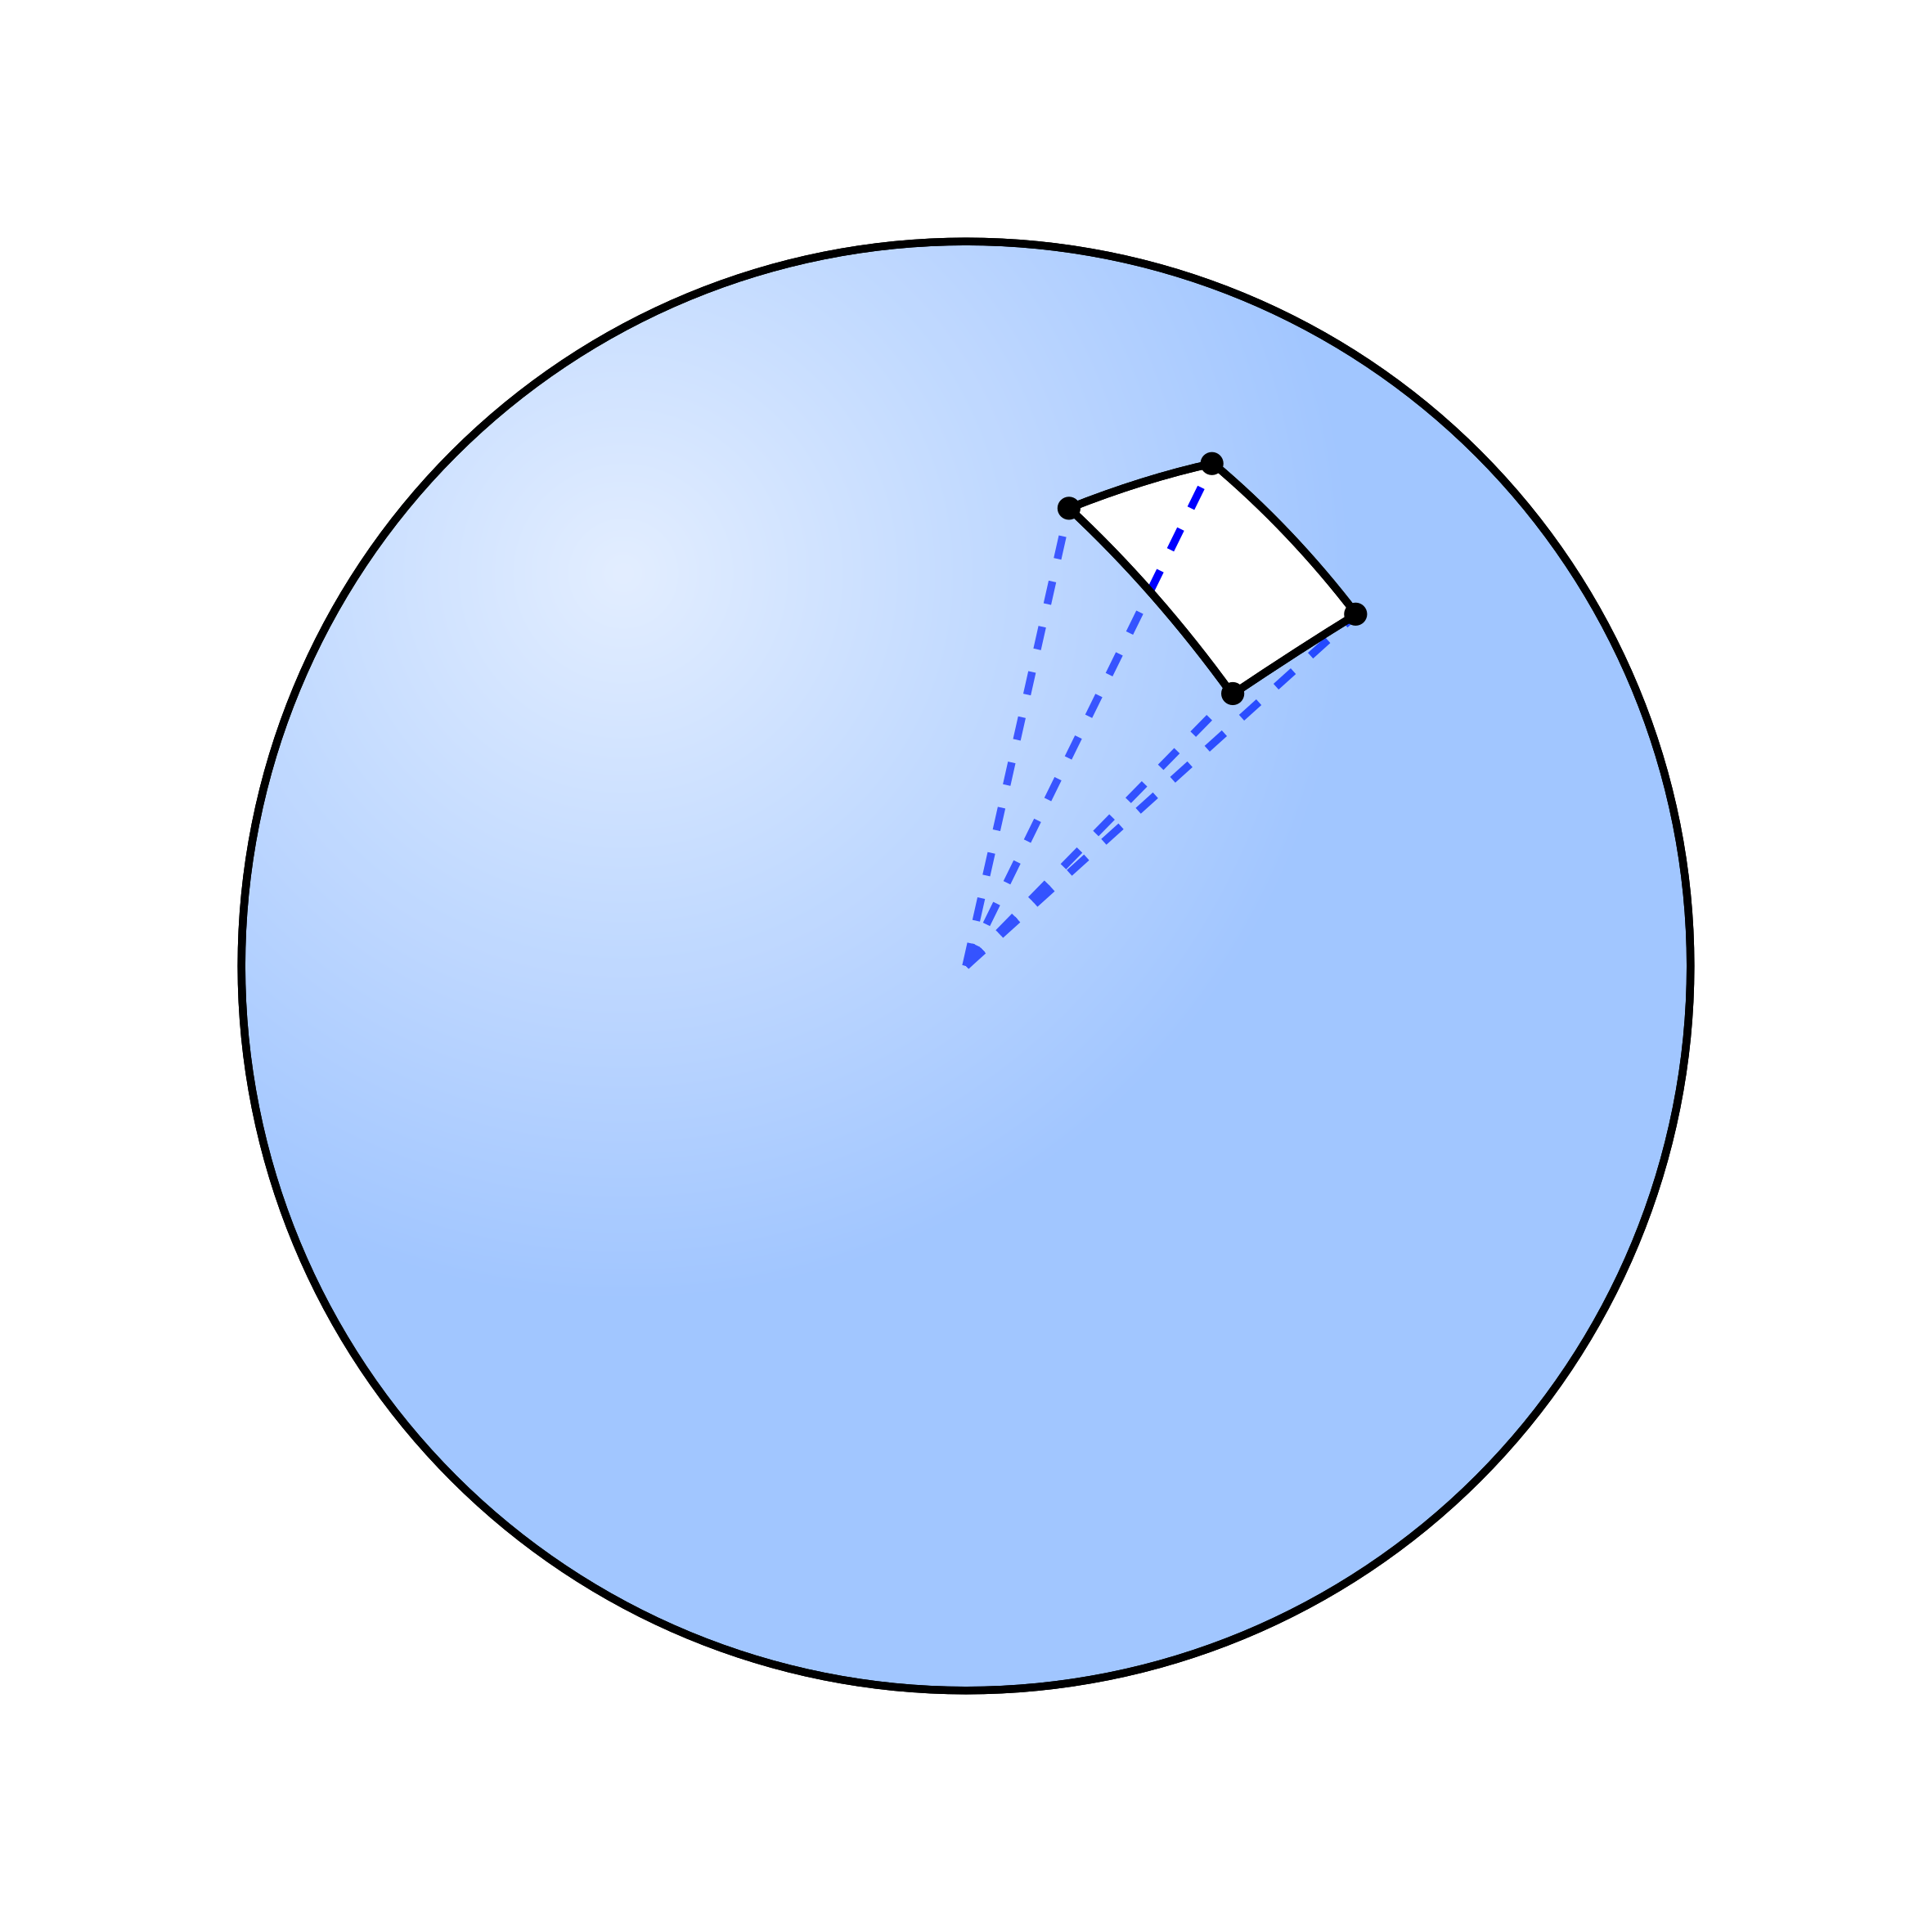
\includegraphics[width=1\textwidth]{inside-outside-1.png} 
	\caption{Wider Area}
	\label{fig:inside_polygon_2}
    \end{minipage} 
\end{figure}



    \item[Swath] The last Cesium object that is currently handled are ground or
	access swaths. The distinction here between \gls{fov} and \gls{for} is
	unimportant since both are displayed in the same way. Swaths are
	displayed with polygons but how this data is generated can be tricky.
	From the \glspl{atu}, swaths are represented through two boundary lines
	that loop around the Earth $L_1$ and $L_2$. These represent the left
	and right boundary of the swath with respect to the velocity vector
	(See section~\ref{sec:atu}).  Typically, to display a swath all that we
	must do is reverse $L_1$ and append it to $L_2$. In this way, we create
	a counter-clockwise ordered polygon that can be displayed on Cesium.
	But, if we do this for a swath that is defined for greater than one
	half-orbit, Cesium will no longer be able to display the polygon
	because it cannot determine what the inside of the polygon is.
	Thankfully, swaths generally only need to be displayed for times where
	a satellite has access to an \gls{aoi}. Automatically sub-dividing
	swaths for longer time ranges will be handled in future iterations of
	\gls{pops}.  Combining the two swaths boundaries is mostly sufficient
	for display purposes but at the beginning and end of a constrained
	swath, we may wish to show the footprint or access region of the
	satellite at the beginning and end of the constrained swath. To do
	this, the \glspl{atu} also provide ellipse representations of the
	footprint/access region for each point in an Ephemeris.  From this
	list, we can take the ellipsoids at the beginning and end of the
	constrained swath, take only the points that lie outside of the swath
	area, and append them to the boundary lists.  That is, 

	\begin{equation*} 
	    P_{swath} = L_1' + E_{start} + L_2 + E_{end} 
	\end{equation*} 

	where $P_{swath}$ is the swath polygon, $L_1'$
	is $L_1$ reversed, and $E_{start}/E_{end}$ are the ellipse points at
	the beginning and end of the constrained swath. Note that the $+$
	symbols here infer list concatenation rather than addition. Calculating
	$E_{start}/E_{end}$ is somewhat involved and is discussed in
	Algorithm~\ref{alg:ellipse}.
	
\begin{figure}
    \centering
    \begin{subfigure}[b]{0.45\textwidth}
	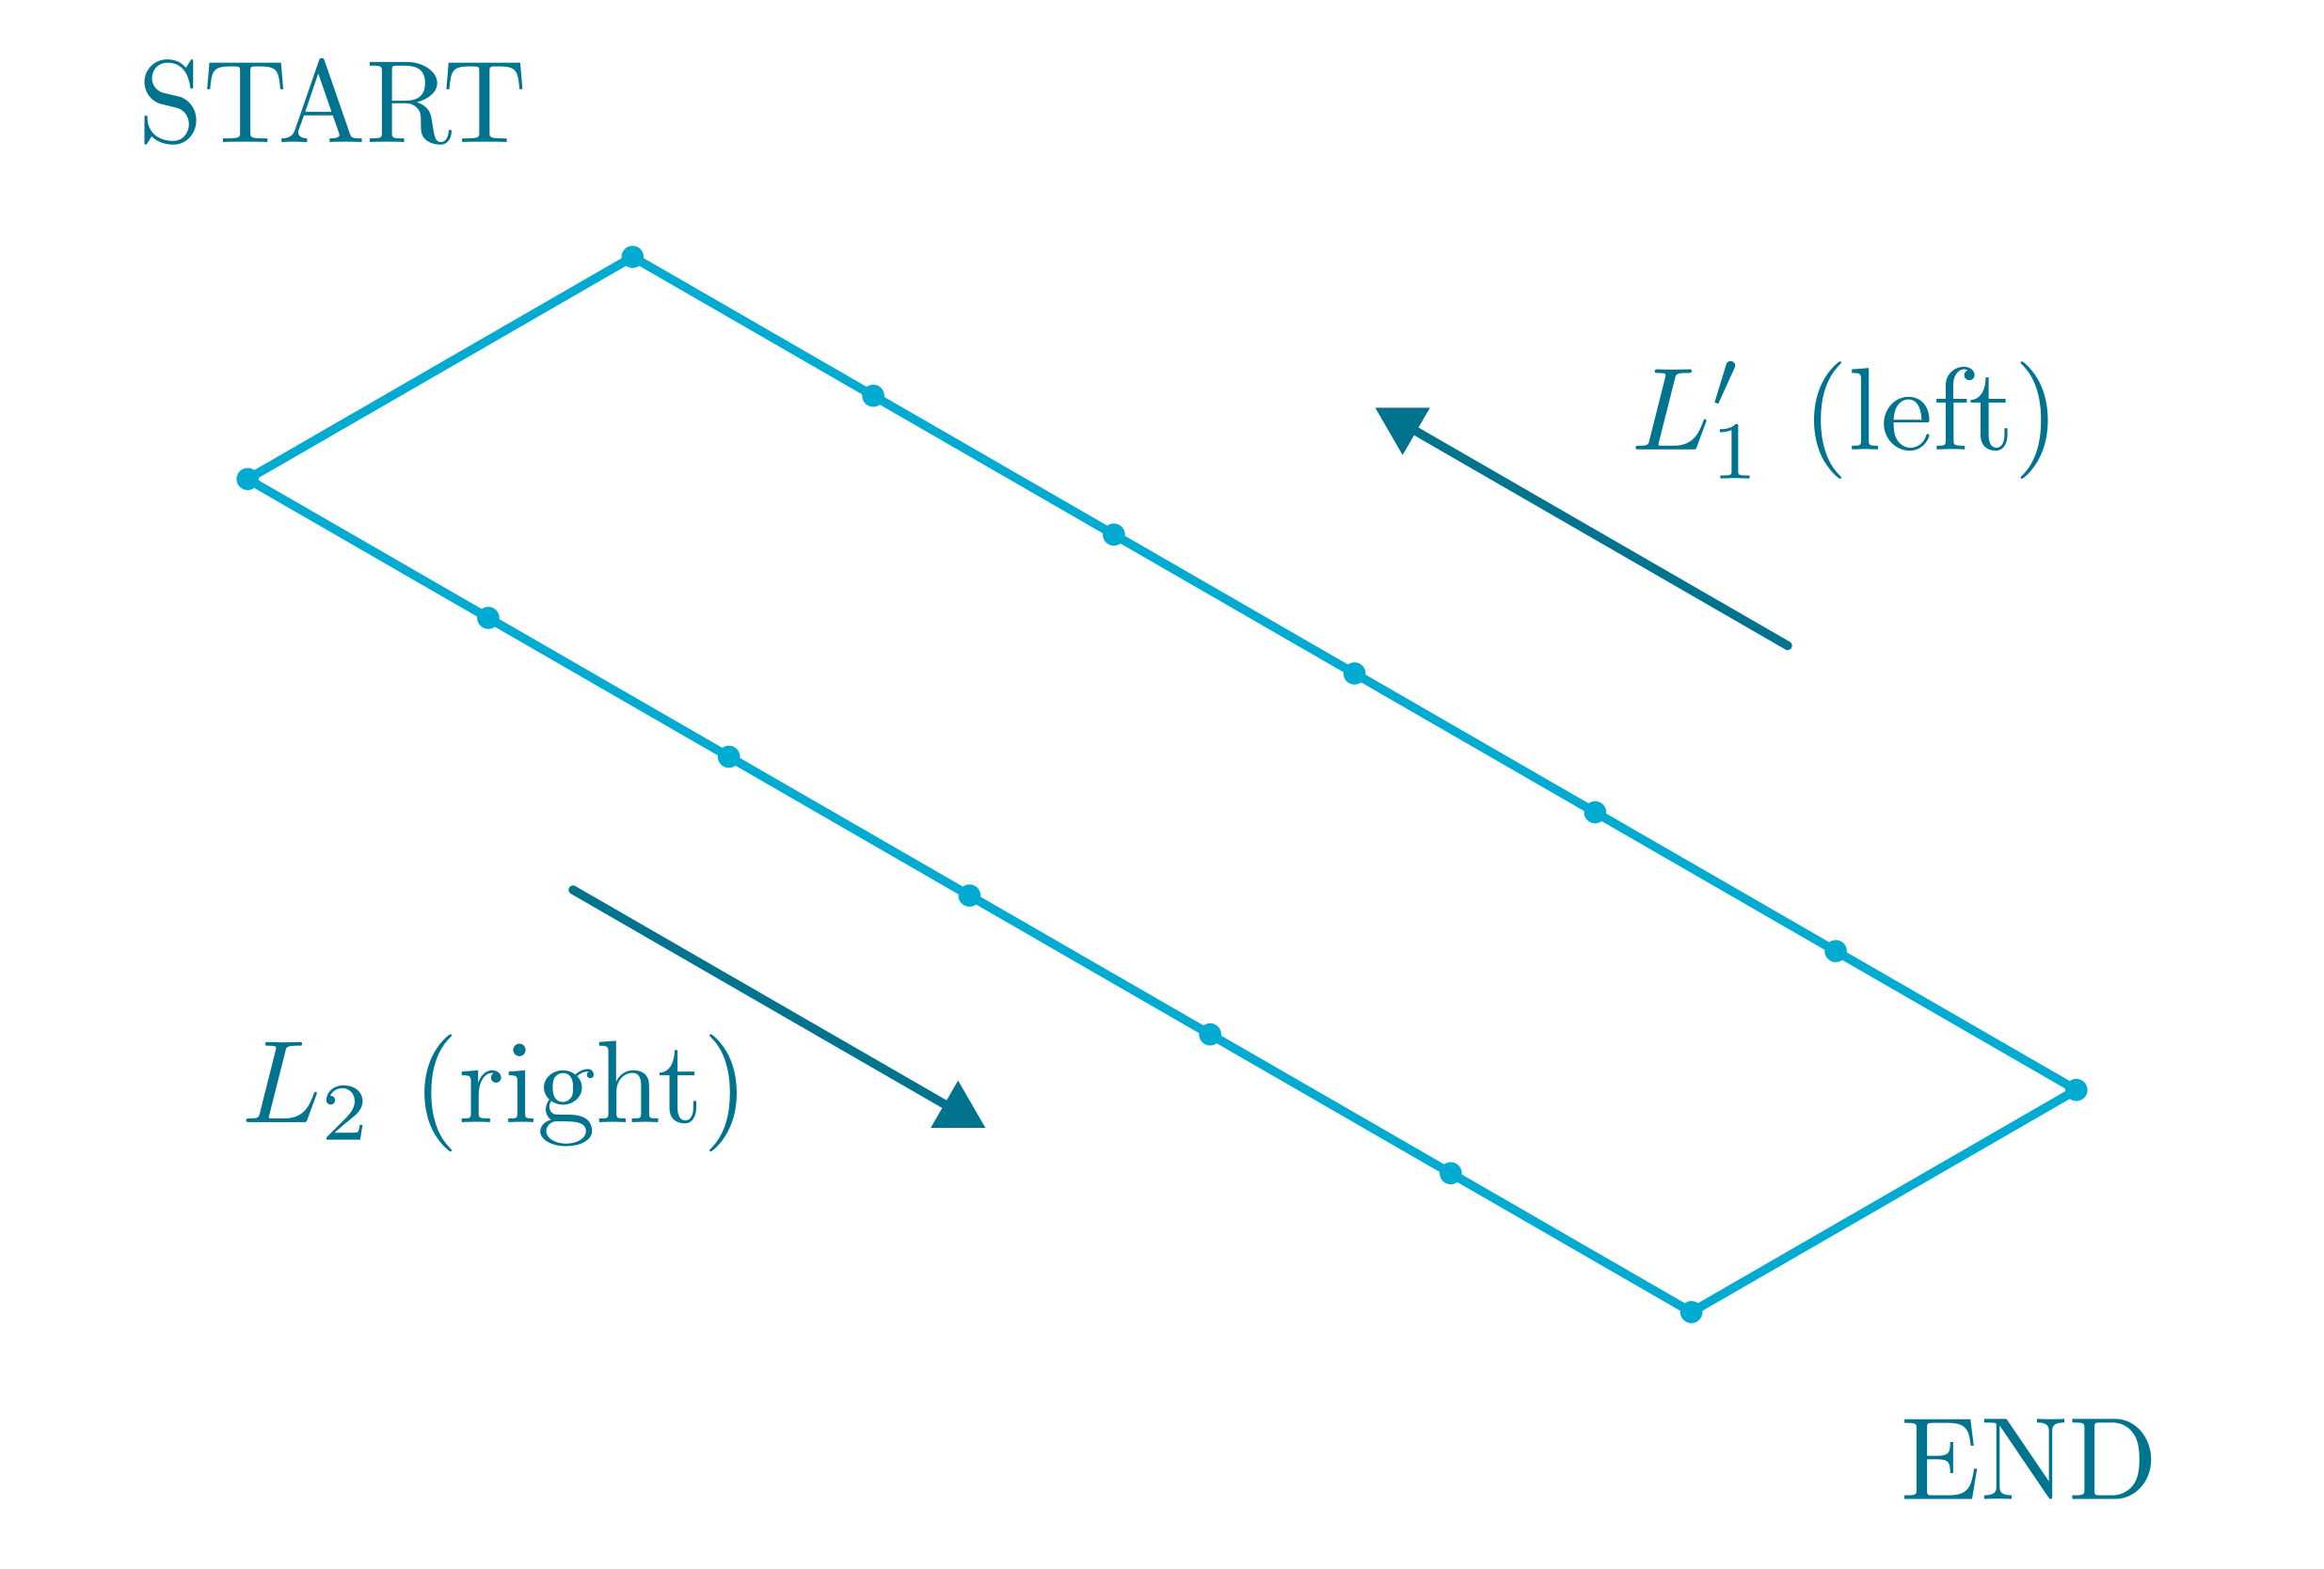
\includegraphics[width=\textwidth]{Swath-1.png} 
	\caption{Basic Swath}
	\label{fig:swath-1}
    \end{subfigure}
    \hfill
    \begin{subfigure}[b]{0.45\textwidth}
	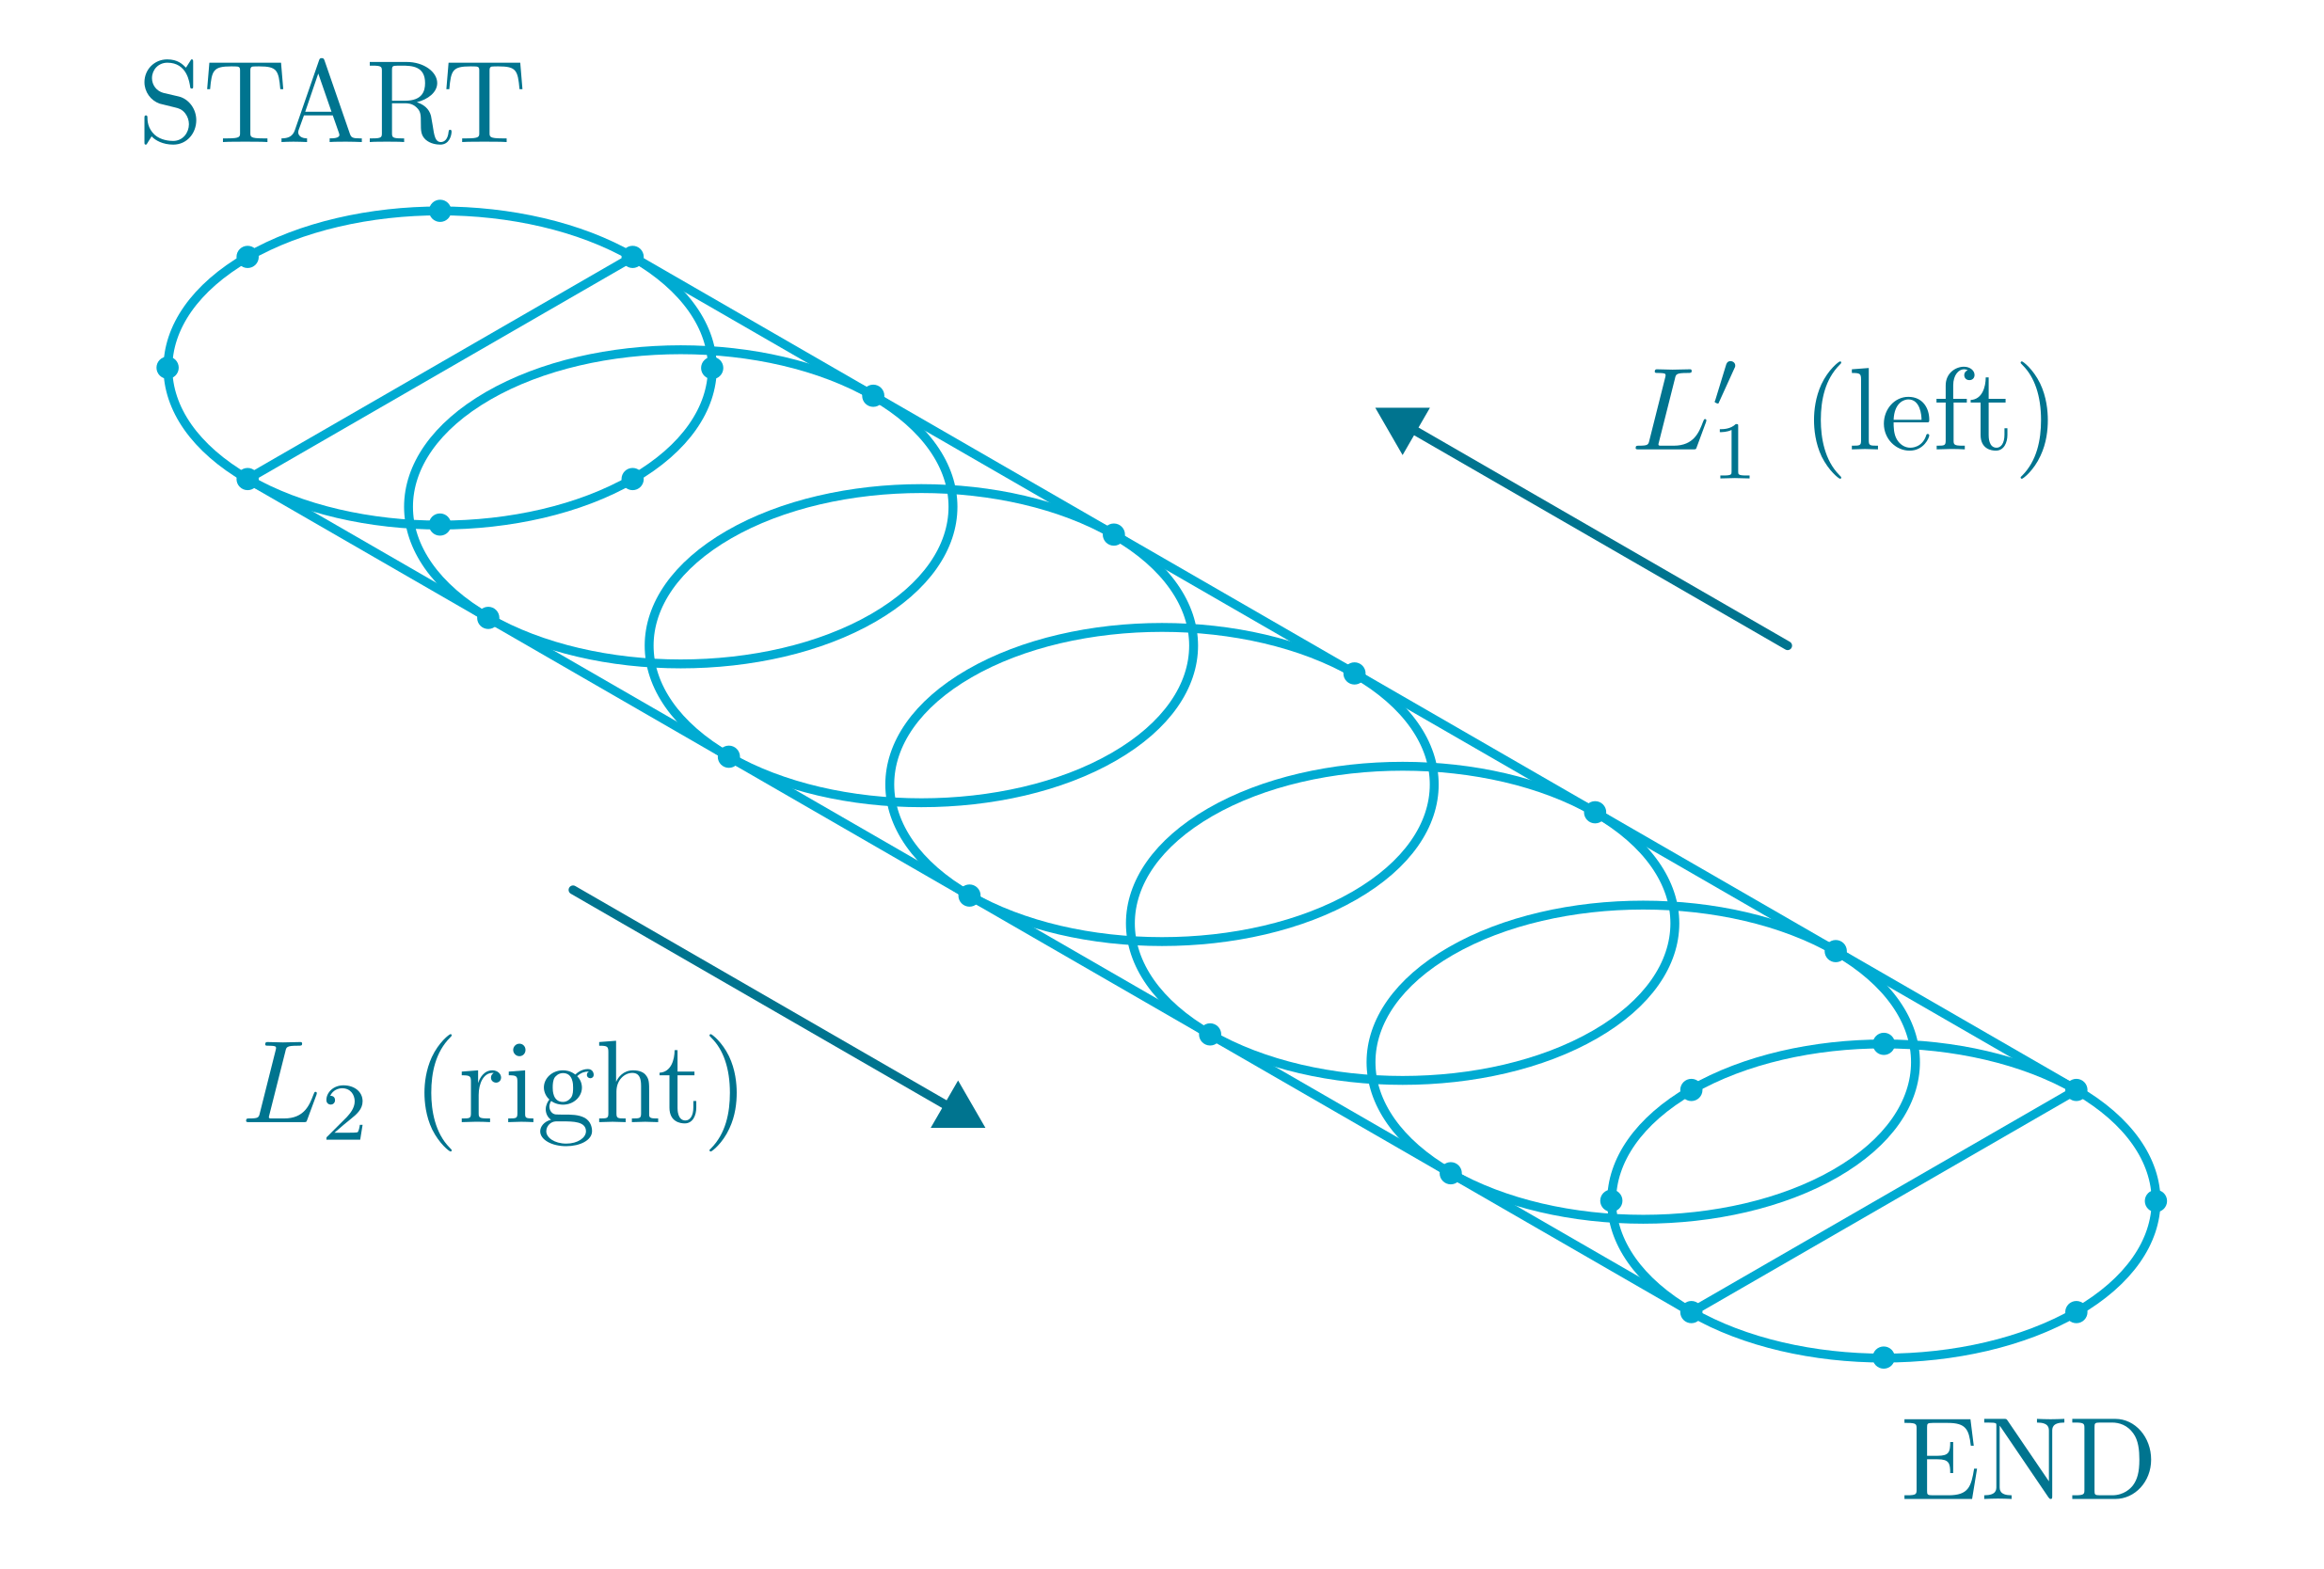
\includegraphics[width=\textwidth]{Swath-2.png} 
	\caption{Footprint/Access Region for each point}
	\label{fig:swath-2}
    \end{subfigure}
    \begin{subfigure}[b]{0.45\textwidth}
	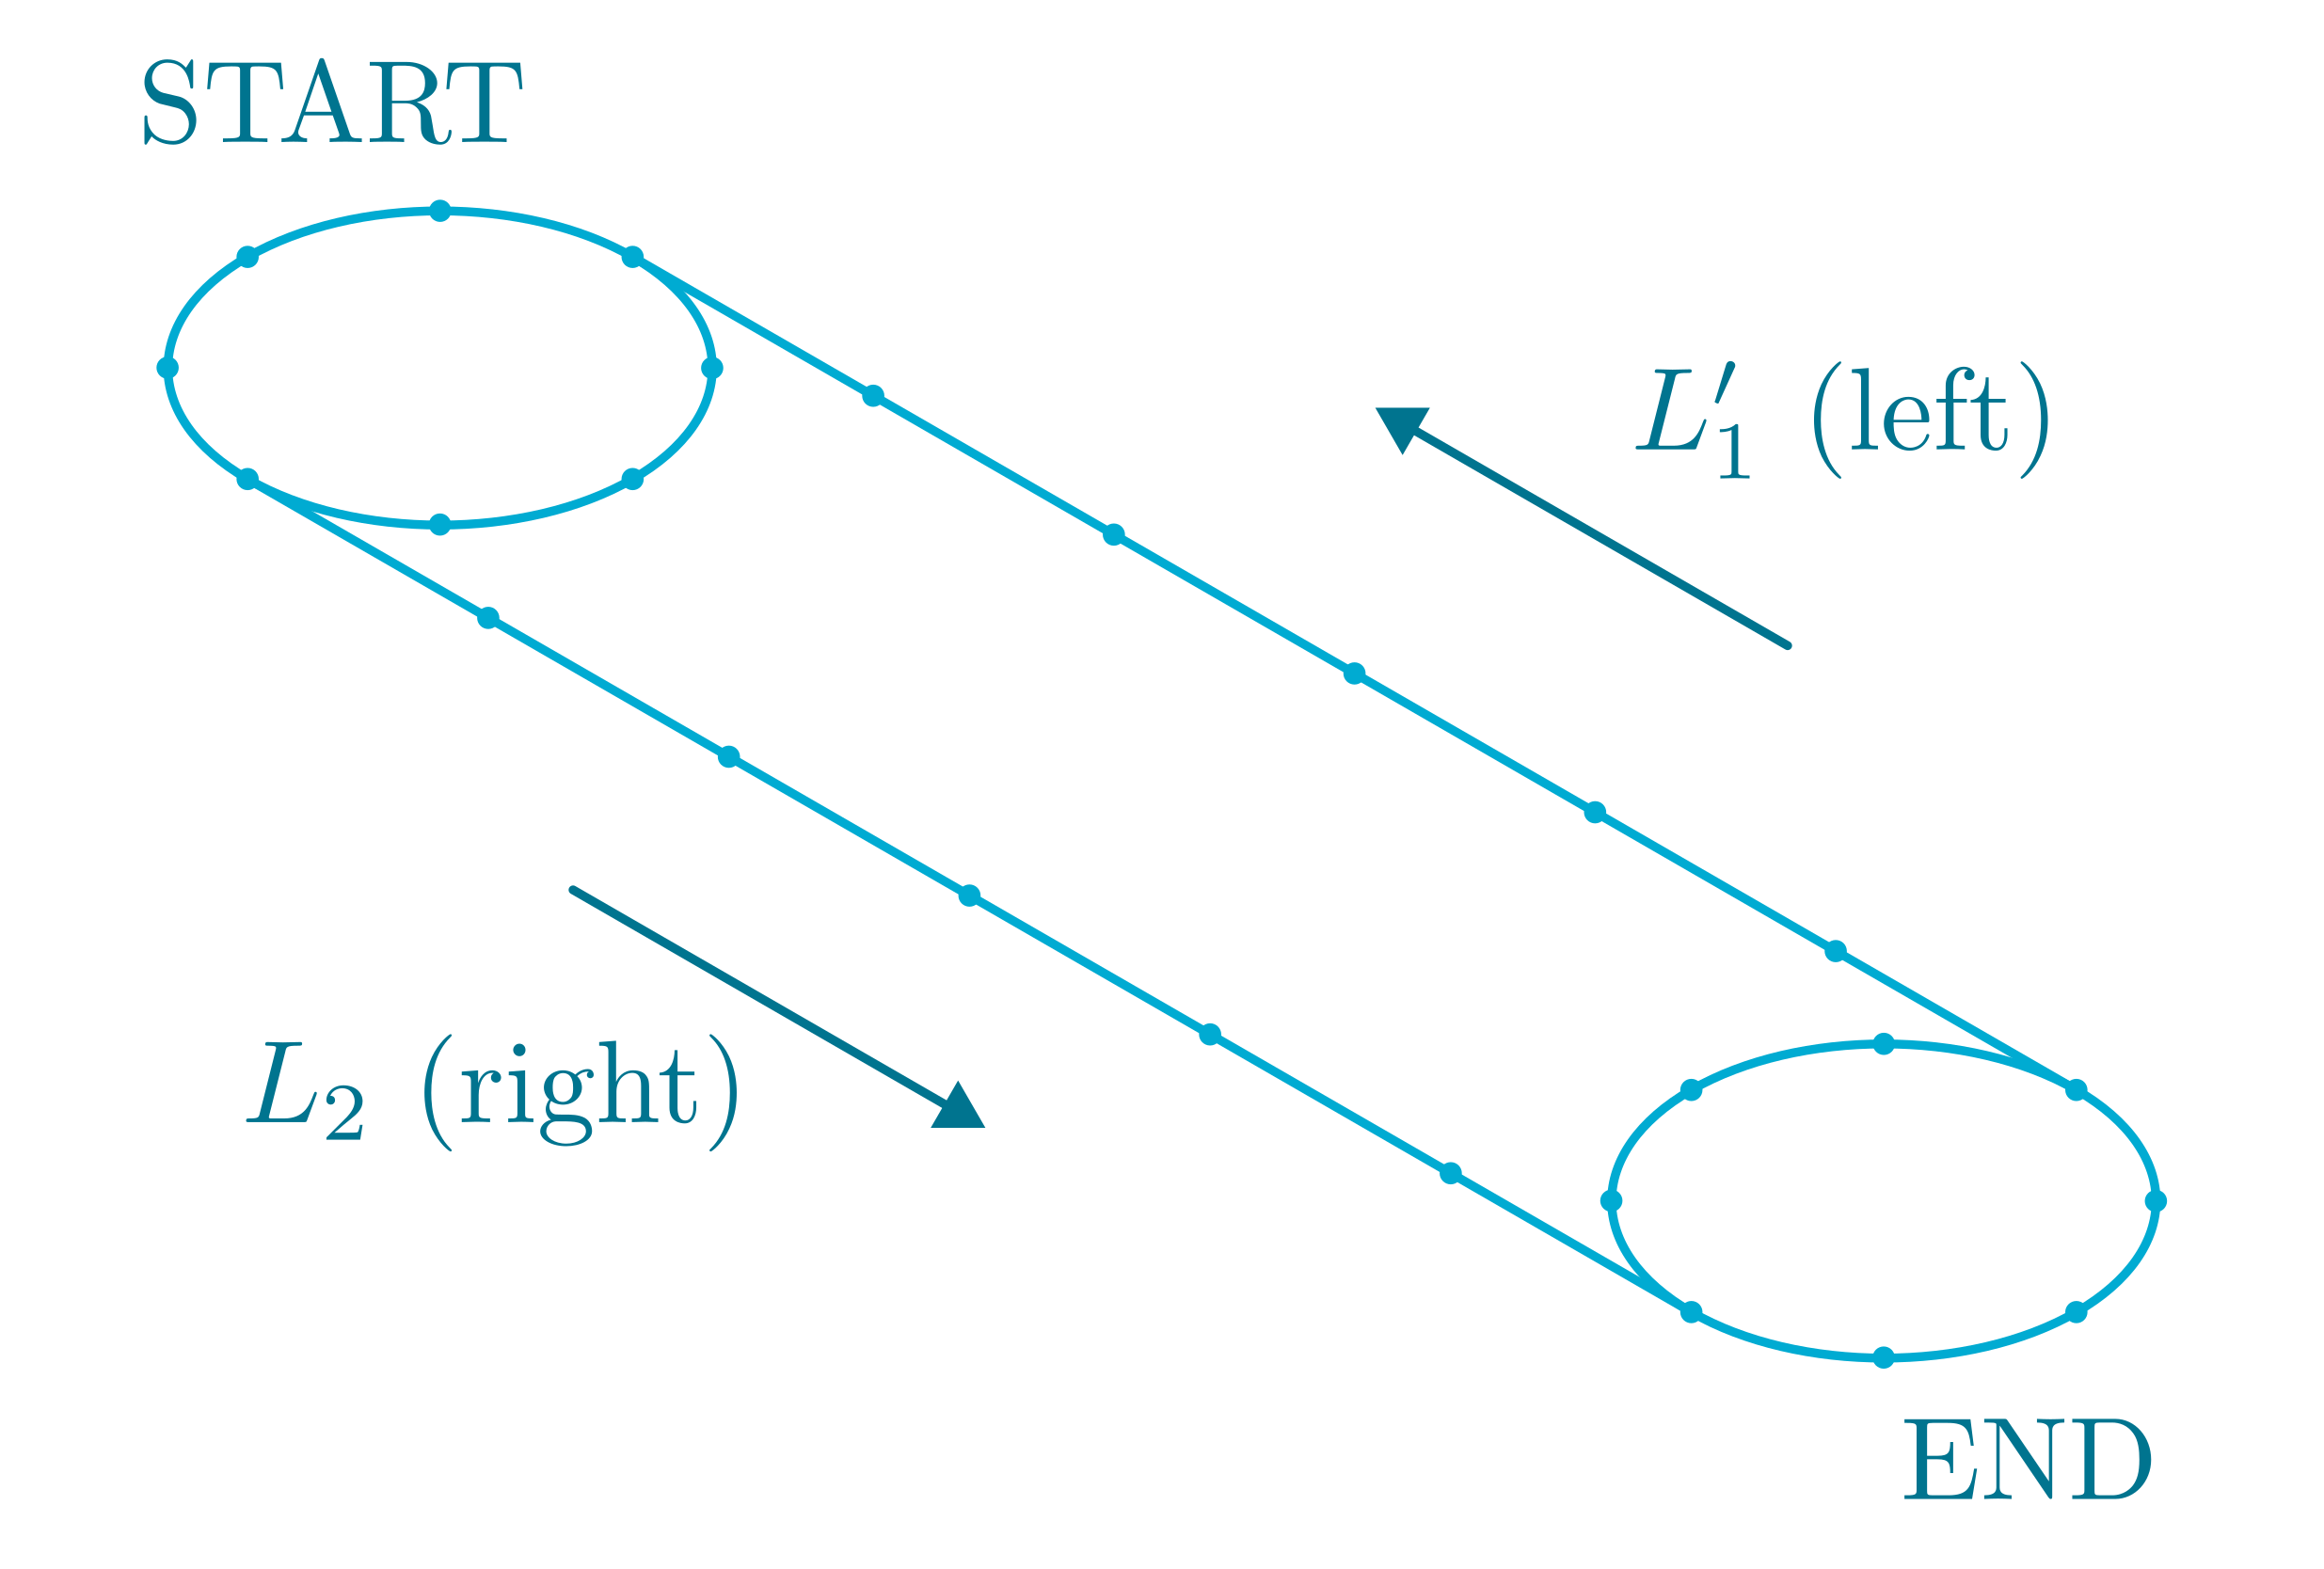
\includegraphics[width=\textwidth]{Swath-3.png} 
	\caption{Start and End Ellipses}
	\label{fig:swath-3}
    \end{subfigure}
    \hfill
    \begin{subfigure}[b]{0.45\textwidth}
	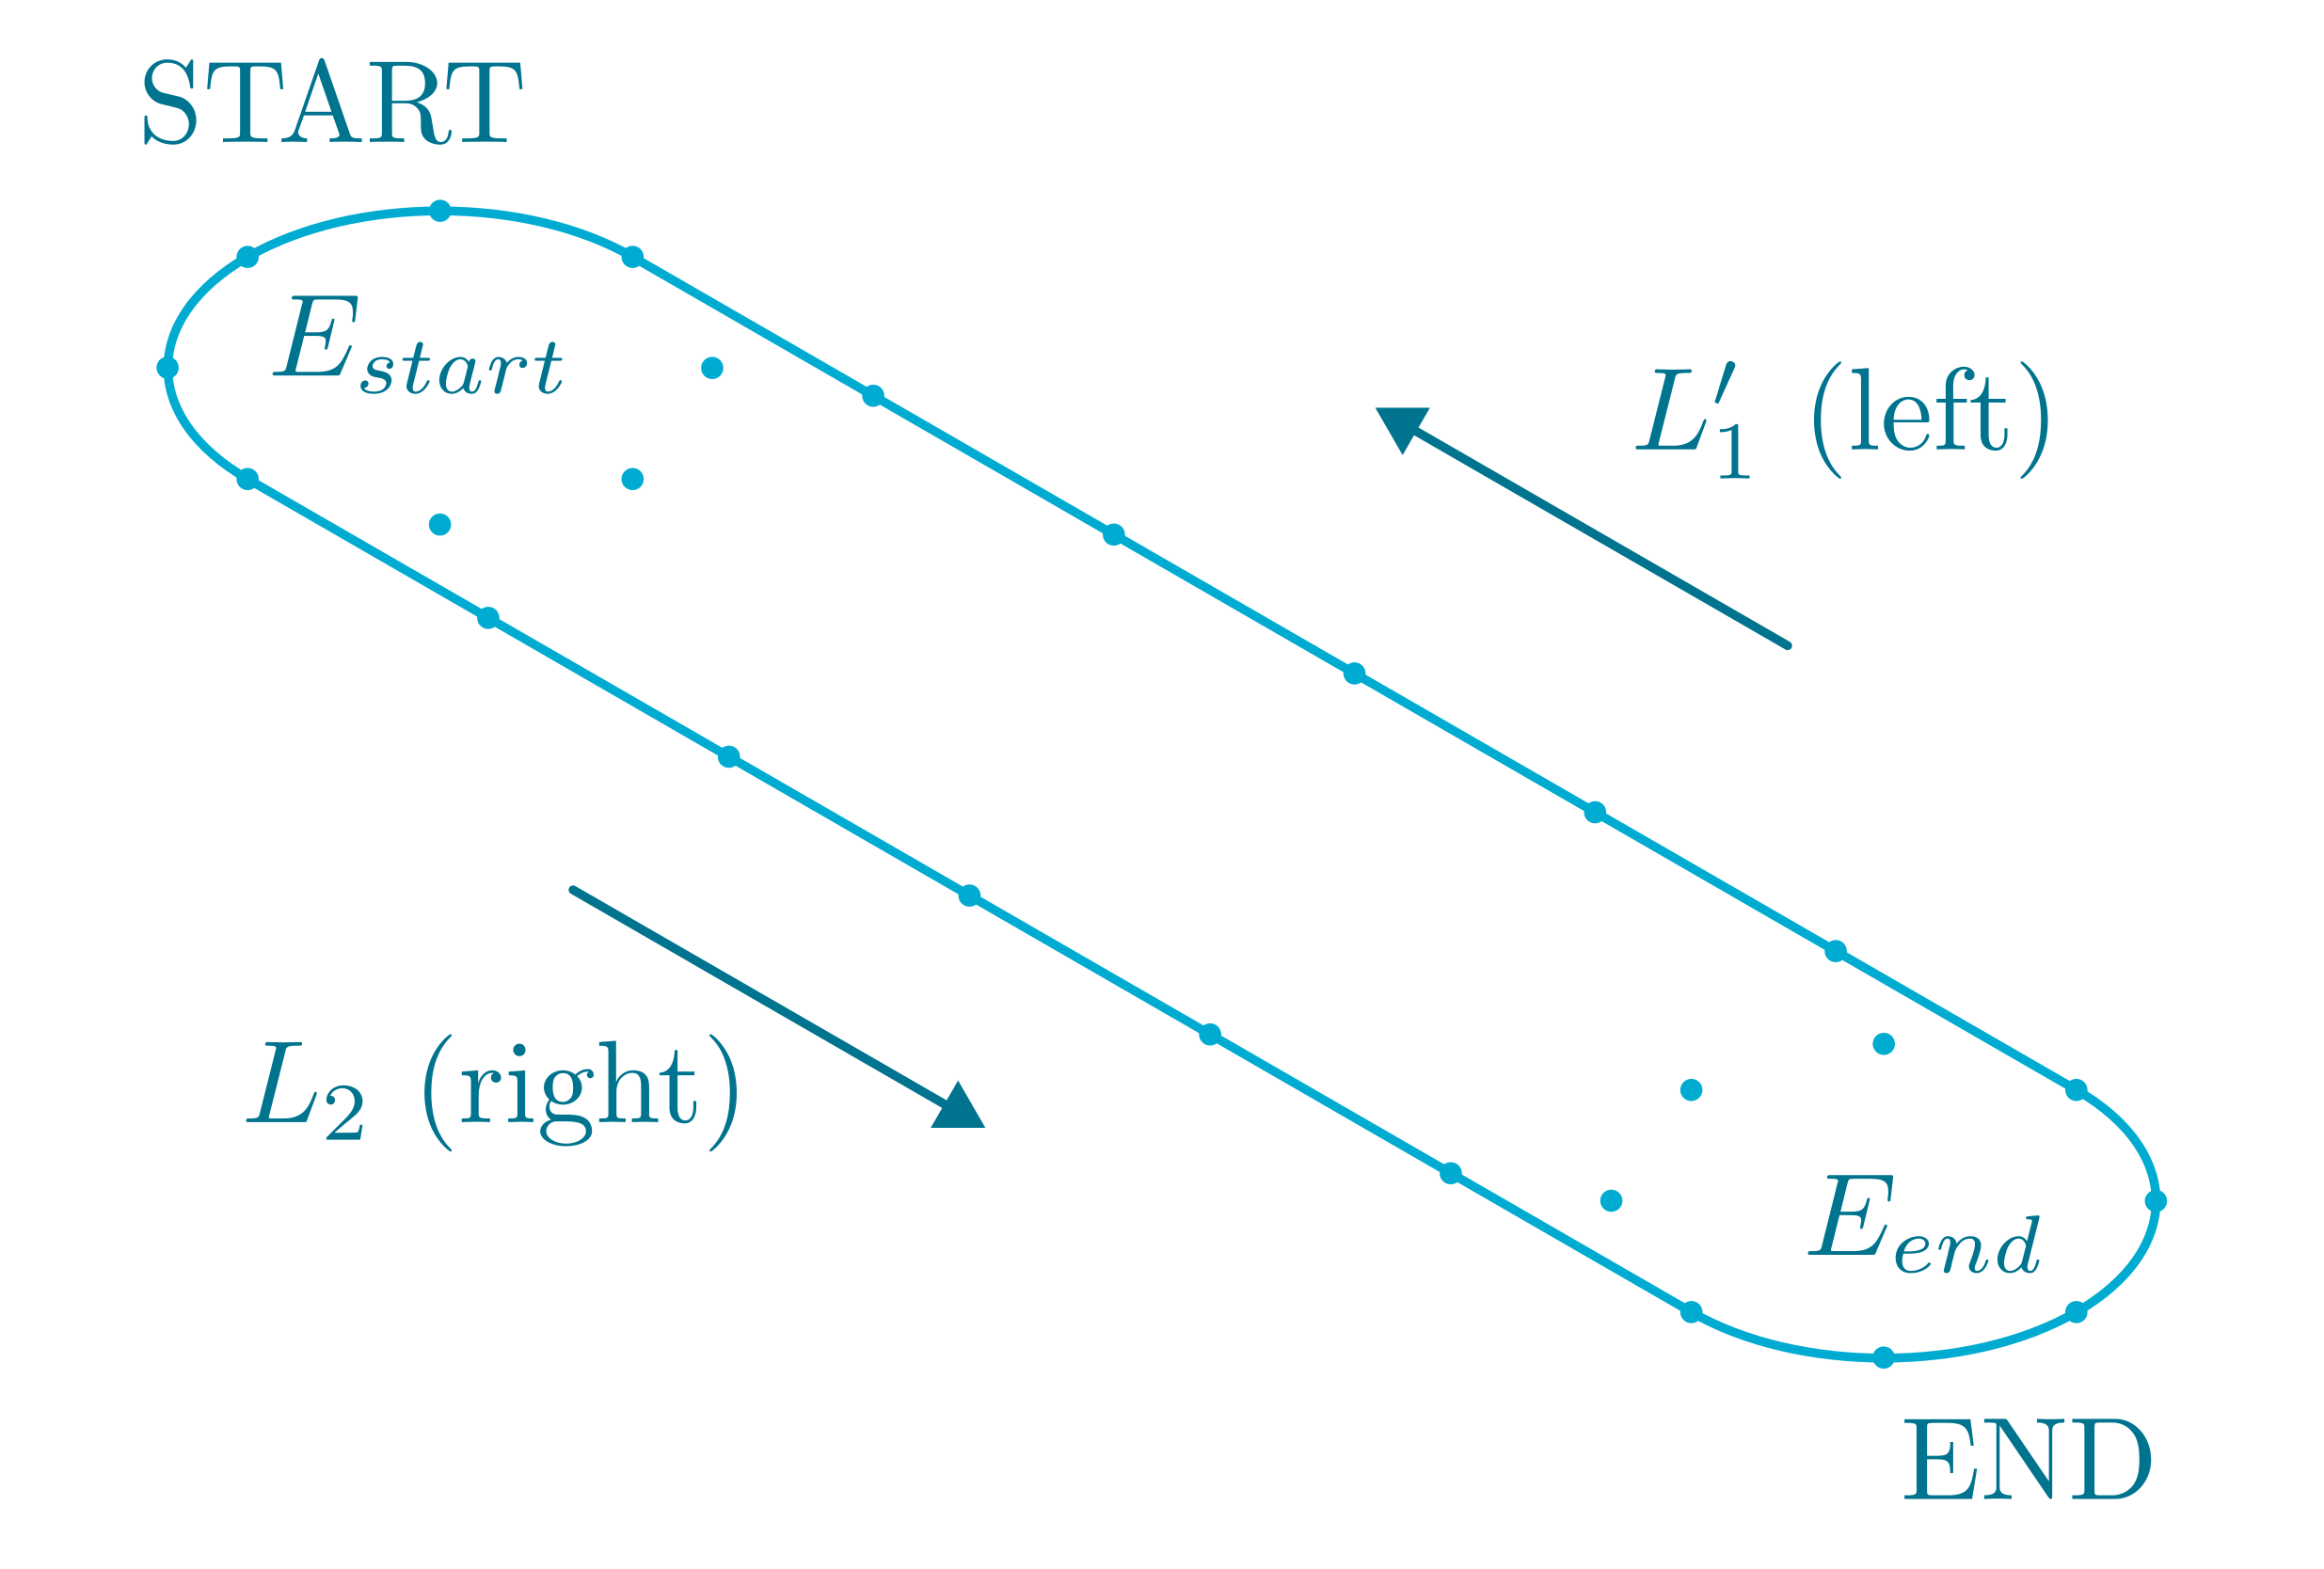
\includegraphics[width=\textwidth]{Swath-4.png} 
	\caption{Final Rounded Swath}
	\label{fig:swath-4}
    \end{subfigure}

    \caption{Steps to display a rounded swath}
    \label{fig:swath-steps}
\end{figure}


\begin{figure}[h]
    \centering
    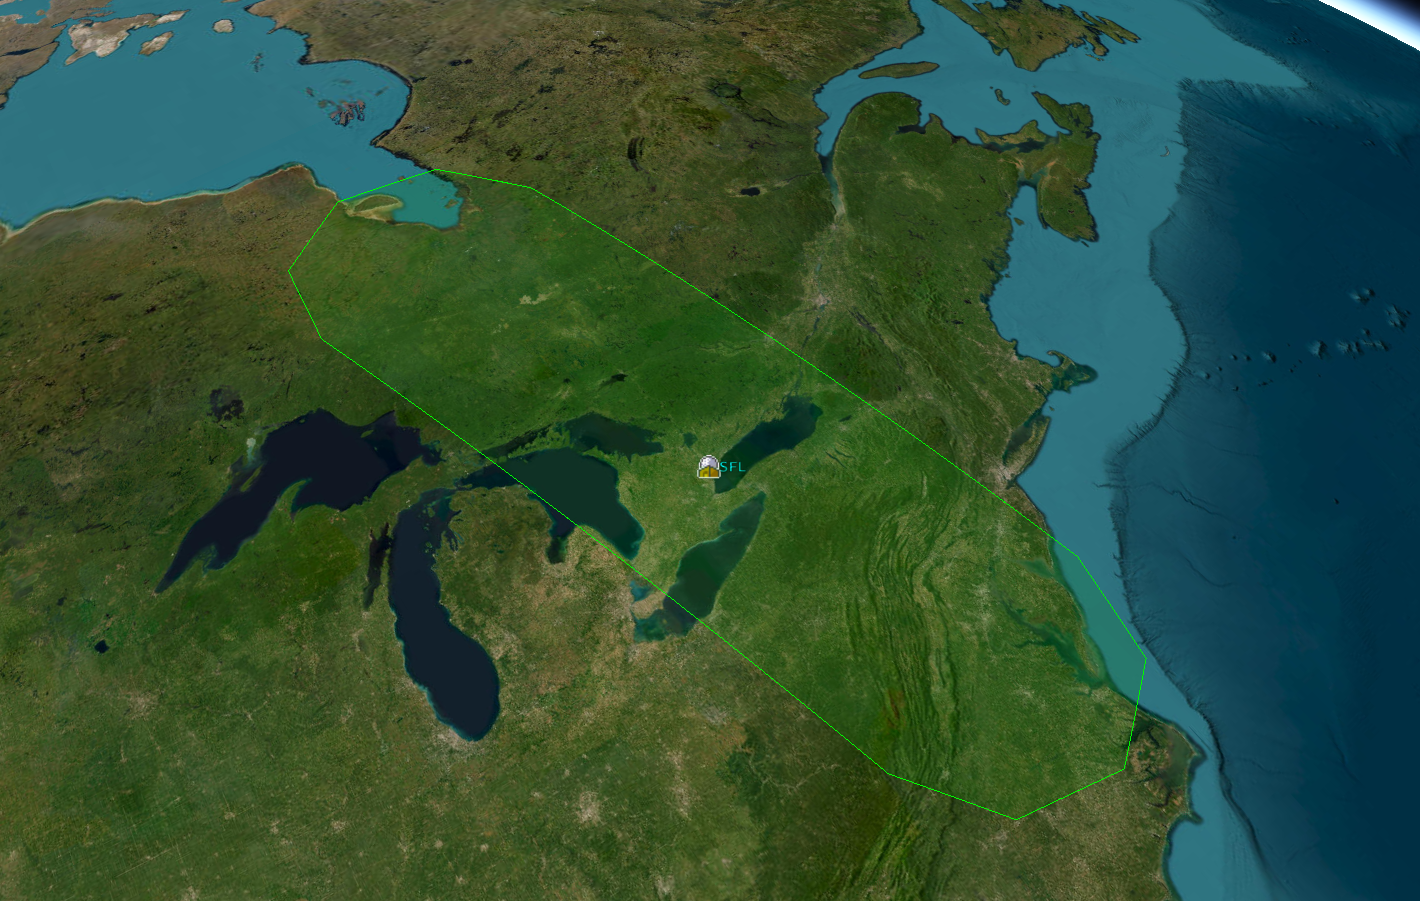
\includegraphics[width=0.9\textwidth]{Cesium_Example_Swath.png} 
    \caption{Example of a 30$^\circ$ Ground Swath}
    \label{fig:cesium_swath}
\end{figure} 

To illustrate this process, see Figure~\ref{fig:swath-steps}.  In
Figure~\ref{fig:swath-1}, we begin a with a simple swath which is just
described by the two boundaries. For each timestep in the swath, the
corresponding footprint/access regions are provided, which can be seen in
Figure~\ref{fig:swath-2}.  From this list, only the start and end ellipses are
selected, Figure~\ref{fig:swath-3}. Finally, these are inputted into
Algorithm~\ref{alg:ellipse} and the results are combined and outputted to
Cesium. An example of a swath being displayed in cesium can be seen in
Figure~\ref{fig:cesium_swath}. 

\end{description}


\subsection{Cesium Handler}

Now that we have an understanding for all of the basic objects that are
supported by \gls{pops}, we may now discuss how they are combined to display
mission information to a user. For this, a Python Cesium Handler class has been
written that acts as the interface between the Python backend and the Cesium
viewer frontend. The Cesium Handler class: keeps track of the entities
currently in the Cesium viewer, keeps track of what entities have been changed
or that need to be updated, and generates new \gls{czml} data to be sent to the
viewer. When the \texttt{main} script is first run, it creates an instance of
the Cesium Handler class as a global variable. In this way it can be referenced
as needed by any \gls{api} call. Some libraries do exist that perform this
functionality but \gls{pops} has enough custom entities that an equivalent
amount of development would need to be done to support them anyway.

To keep track of entities in the viewer, the Cesium Handler class has a list of
objects where each object is a Cesium Model. As such, it has all of the meta
information of the \texttt{BaseObject} as well as a method to build a
\gls{czml} packet and delete packet. By setting up Cesium objects in this way,
they can be treated completely generally by the Cesium Handler class and
metadata can be stored and referenced for every object. This metadata tracks
the status of Cesium objects and determines whether any changes need to be made
in the viewer. 

Objects can be added or removed with helper functions in the Cesium Handler
class. Either objects can be added directly by creating an instance of a Cesium
Model class, then appending them to the list of objects in the Cesium Handler
or a developer can use one of the helper methods. Some situations may require
specific logic to set up a scenario. This is the case for displaying search
scenarios or adding opportunities to a viewer. Currently, there is no way to
generally display the results of a search scenario. A developer must explicitly
define what swaths, intersection polygons, or \glspl{aoi} to add. In the
future, this may be made completely general through some sophisticated
implementation but the current method is sufficient. As with the database,
opportunities are also linked in the Cesium Handler class so that they can be
referenced and enabled or disabled as desired. This makes visualizing search
scenarios much more clear. 

To actual effect changes to the Cesium viewer, the Cesium Handler makes use of
an asynchronous approach. A user may make a change to the viewer at any time or
they may even make many changes in quick succession and the viewer must be able
to update correctly. Whenever a change is made to the objects list, first,
\gls{czml} packets are generated for each object whose \texttt{changed} flag is
raised. In this way \gls{czml} is only sent when necessary and the viewer is
not bombarded with duplicate data. These packets are then added to a queue and
a flag is raised in the Cesium Handler class to signal that packets are ready
to be sent to the Cesium viewer. Within the Mission Model's main script there
is a loop that checks for this flag. Once it is raised, the main script sends
every \gls{czml} packet in the queue to the viewer and then verifies that the
correct number of packets were received in a return message. If the validation
passes, then the changed flag is reset for all of the objects that were
processed; otherwise, the requests are sent again. The reason for using a queue
is that it allows for many requests to be processed in the order that they are
added.  Not controlling this may lead to undefined behavior if the rate at
which changes are made faster than they can be effected in the viewer.


\subsection{Scheduler}

The last component of the Mission Model that should be discussed is the
Scheduler class. The purpose of this class is to keep track of what
observations are planned for all the satellites that are being tracked by
\gls{pops}. The class should be able to: store satellite events, validate
schedules based on some ruleset, and must be able to display all events in a
timeline to the user. 

The base unit for the schedule class are Events. An Event is a general object
that can be used to describe anything. Every Event contains two categories of
data. They have data that is universal to all Events and a payload which is
Event specific.  The universal data describes information about the object
itself, such as:

\begin{description} 

    \item[ID] The ID of an Event which is either a serial number or an
	enumerated descriptive name.

    \item[Name] This is what is actually displayed to the user and may have
	more information than just an ID.

    \item[Type] Is the Event a station keeping maneuver, a planned observation,
	a ground contact, etc. The type is arbitrary but it allows Events to be
	filtered or treated in different ways based on this value.

    \item[Satellite] Each Event must be associated with a single satellite. If
	multiple satellites are undergoing the same event, each will have their
	own Event object.

    \item[Time Data] Information such as the start, stop, and epoch of an
	Event. An epoch can mostly be ignored but it is important for when
	\glspl{ttc} are created. This is discussed in the \gls{ttc} generation
	section, Section~\ref{sec:ttc-gen}.

    \item[Linked Events] For the case where multiple Events are related in some
	way, they may be linked together. One use for this is if one Event is
	deleted, all other linked Events are deleted as well.

\end{description} 

Along with each Event is a payload. The payloads allow for specific information
to be stored in an Event without the Scheduler class being aware of what's
there. This functionality will primary be used to contain observation-specific
information such that \glspl{ttc} can be generated from lists of Events without
having the Scheduler class be aware of what observations are possible.
Observations are just one example of an Event. In the future, there may be some
other type of Event a developer may wish to store information in.  It should be
noted that the Scheduler class will never access or manipulate an Event's
payload except to display the information to a user.

A `schedule' is a universal concept. A satellite has one and only one timeline.
This means that, the scheduler class exists outside off plans or observation
configuration. A plan may add Events to a schedule or certain Events may be
relevant in a plan but ultimately Events and the timeline exist outside of any
given plan. This is all to say that when a timeline is displayed to a user,
only the parts of the schedule that are relevant to the plan are visible.
Events are filtered by satellites, time ranges, or type. If Events are added to
the schedule by a plan, those Events now exist universally for any plan. There
does not exist one schedule for one plan, it is all the same schedule.

With this universality in mind, it follows that the Scheduler class has a
1-to-1 relationship with the database. Within the database there is a table of
Events and within the scheduler class there is a list of Events. Every time an
Event is added to the list of Events, a corresponding row is added to the
Database. When the Scheduler class is instantiated, it immediately loads all of
the Events currently stored in the database to its list of Events. The purpose
of this is that \gls{pops} may be shutdown at any time and the list of Events
is retained in the database. By design, there exists no situation where the
Scheduler class differs from the Database.

The Scheduler class also has the ability to validate schedules based on a
library of rulesets. These rulesets are separate add-ons to the Scheduler
class. Within the class, their is a \texttt{validate\_schedule()} method, which
passes the list of Events to every ruleset. These rulesets then return lists of
conflicts. These conflicts are stored and displayed to the user graphically and
in a list. The reason why rulesets are treated in this way, is that it allows
the Scheduler class to be expandable. Currently, there is only one ruleset and
it checks for time conflicts. For a satellite, it checks whether there exist
instances where 2 or more Events are scheduled to happen at the same time.
This is a very basic rule, and it stems from the fact that a satellite cannot
be commanded to do more than one thing at once (at least at this early stage of
development).  In the future, there will be more rulesets.  For example the
schedule: must not exceed a satellite's data budget, must conform with a
satellite's attitude control constraints, check if Events are possible with
updated weather reports, etc.

Though not currently supported, it is planned that an interface will be
developed that allows Events to be generated from ground software. From a list
of \glspl{ttc} that have been uploaded to a satellite, Events will be generated
in the schedule to represent them. In this way, a \gls{pops} user will be able
to see what \glspl{ttc} are already planned for a given satellite. This will
help them develop an operations strategy. This functionality will also expand
the usefulness of \gls{pops} beyond just planning.

%% TODO: Add observations to timeline
\begin{figure}
    \centering
    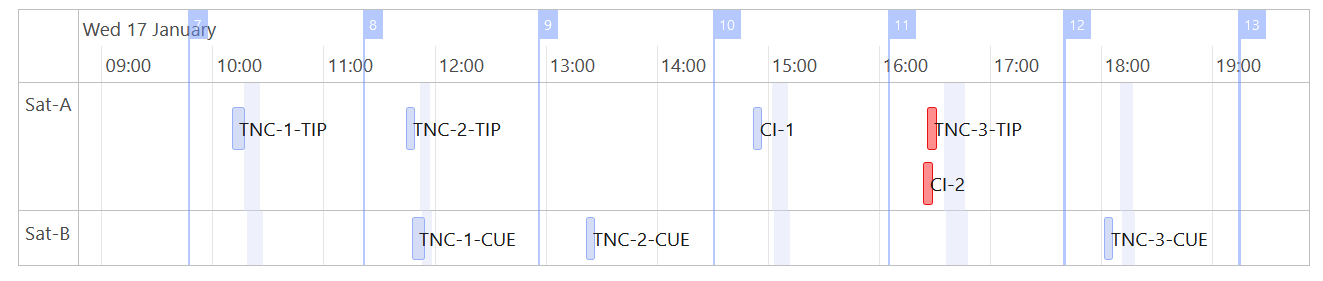
\includegraphics[width=1\textwidth]{timeline-example-2.png} 
    \caption{Example of a Timeline}
    \label{fig:scheduler-timeline}
\end{figure}

The last functionality of the Scheduler class is visualizing a schedule in a
timeline. To do this, the Scheduler class will take a list of Events, filter
them based on the visualization request, format them into a large data packet,
and pass that packet to the webpage. On the webpage, an open-source library is
used to format the timeline. An example of a timeline can be seen in
Figure~\ref{fig:scheduler-timeline}. Observations for each satellite are split
into rows. Events are displayed as blue boxes with descriptive names.
Conflicting Events are shaded in red. To give more information to the user, the
pass boundaries are displayed as blue vertical lines. The shaded regions
specify when a satellite has access to a ground station.  Currently, this is
all that is displayed is subject to change based on feedback from operators
using the tool.



%\section{NSP Service}







